% Options for packages loaded elsewhere
% Options for packages loaded elsewhere
\PassOptionsToPackage{unicode}{hyperref}
\PassOptionsToPackage{hyphens}{url}
\PassOptionsToPackage{dvipsnames,svgnames,x11names}{xcolor}
%
\documentclass[
  letterpaper,
  DIV=11,
  numbers=noendperiod]{scrartcl}
\usepackage{xcolor}
\usepackage{amsmath,amssymb}
\setcounter{secnumdepth}{-\maxdimen} % remove section numbering
\usepackage{iftex}
\ifPDFTeX
  \usepackage[T1]{fontenc}
  \usepackage[utf8]{inputenc}
  \usepackage{textcomp} % provide euro and other symbols
\else % if luatex or xetex
  \usepackage{unicode-math} % this also loads fontspec
  \defaultfontfeatures{Scale=MatchLowercase}
  \defaultfontfeatures[\rmfamily]{Ligatures=TeX,Scale=1}
\fi
\usepackage{lmodern}
\ifPDFTeX\else
  % xetex/luatex font selection
\fi
% Use upquote if available, for straight quotes in verbatim environments
\IfFileExists{upquote.sty}{\usepackage{upquote}}{}
\IfFileExists{microtype.sty}{% use microtype if available
  \usepackage[]{microtype}
  \UseMicrotypeSet[protrusion]{basicmath} % disable protrusion for tt fonts
}{}
\makeatletter
\@ifundefined{KOMAClassName}{% if non-KOMA class
  \IfFileExists{parskip.sty}{%
    \usepackage{parskip}
  }{% else
    \setlength{\parindent}{0pt}
    \setlength{\parskip}{6pt plus 2pt minus 1pt}}
}{% if KOMA class
  \KOMAoptions{parskip=half}}
\makeatother
% Make \paragraph and \subparagraph free-standing
\makeatletter
\ifx\paragraph\undefined\else
  \let\oldparagraph\paragraph
  \renewcommand{\paragraph}{
    \@ifstar
      \xxxParagraphStar
      \xxxParagraphNoStar
  }
  \newcommand{\xxxParagraphStar}[1]{\oldparagraph*{#1}\mbox{}}
  \newcommand{\xxxParagraphNoStar}[1]{\oldparagraph{#1}\mbox{}}
\fi
\ifx\subparagraph\undefined\else
  \let\oldsubparagraph\subparagraph
  \renewcommand{\subparagraph}{
    \@ifstar
      \xxxSubParagraphStar
      \xxxSubParagraphNoStar
  }
  \newcommand{\xxxSubParagraphStar}[1]{\oldsubparagraph*{#1}\mbox{}}
  \newcommand{\xxxSubParagraphNoStar}[1]{\oldsubparagraph{#1}\mbox{}}
\fi
\makeatother


\usepackage{longtable,booktabs,array}
\usepackage{calc} % for calculating minipage widths
% Correct order of tables after \paragraph or \subparagraph
\usepackage{etoolbox}
\makeatletter
\patchcmd\longtable{\par}{\if@noskipsec\mbox{}\fi\par}{}{}
\makeatother
% Allow footnotes in longtable head/foot
\IfFileExists{footnotehyper.sty}{\usepackage{footnotehyper}}{\usepackage{footnote}}
\makesavenoteenv{longtable}
\usepackage{graphicx}
\makeatletter
\newsavebox\pandoc@box
\newcommand*\pandocbounded[1]{% scales image to fit in text height/width
  \sbox\pandoc@box{#1}%
  \Gscale@div\@tempa{\textheight}{\dimexpr\ht\pandoc@box+\dp\pandoc@box\relax}%
  \Gscale@div\@tempb{\linewidth}{\wd\pandoc@box}%
  \ifdim\@tempb\p@<\@tempa\p@\let\@tempa\@tempb\fi% select the smaller of both
  \ifdim\@tempa\p@<\p@\scalebox{\@tempa}{\usebox\pandoc@box}%
  \else\usebox{\pandoc@box}%
  \fi%
}
% Set default figure placement to htbp
\def\fps@figure{htbp}
\makeatother

\ifLuaTeX
  \usepackage{luacolor}
  \usepackage[soul]{lua-ul}
\else
  \usepackage{soul}
\fi

% definitions for citeproc citations
\NewDocumentCommand\citeproctext{}{}
\NewDocumentCommand\citeproc{mm}{%
  \begingroup\def\citeproctext{#2}\cite{#1}\endgroup}
\makeatletter
 % allow citations to break across lines
 \let\@cite@ofmt\@firstofone
 % avoid brackets around text for \cite:
 \def\@biblabel#1{}
 \def\@cite#1#2{{#1\if@tempswa , #2\fi}}
\makeatother
\newlength{\cslhangindent}
\setlength{\cslhangindent}{1.5em}
\newlength{\csllabelwidth}
\setlength{\csllabelwidth}{3em}
\newenvironment{CSLReferences}[2] % #1 hanging-indent, #2 entry-spacing
 {\begin{list}{}{%
  \setlength{\itemindent}{0pt}
  \setlength{\leftmargin}{0pt}
  \setlength{\parsep}{0pt}
  % turn on hanging indent if param 1 is 1
  \ifodd #1
   \setlength{\leftmargin}{\cslhangindent}
   \setlength{\itemindent}{-1\cslhangindent}
  \fi
  % set entry spacing
  \setlength{\itemsep}{#2\baselineskip}}}
 {\end{list}}
\usepackage{calc}
\newcommand{\CSLBlock}[1]{\hfill\break\parbox[t]{\linewidth}{\strut\ignorespaces#1\strut}}
\newcommand{\CSLLeftMargin}[1]{\parbox[t]{\csllabelwidth}{\strut#1\strut}}
\newcommand{\CSLRightInline}[1]{\parbox[t]{\linewidth - \csllabelwidth}{\strut#1\strut}}
\newcommand{\CSLIndent}[1]{\hspace{\cslhangindent}#1}



\setlength{\emergencystretch}{3em} % prevent overfull lines

\providecommand{\tightlist}{%
  \setlength{\itemsep}{0pt}\setlength{\parskip}{0pt}}



 


\KOMAoption{captions}{tableheading,figureheading}
\makeatletter
\@ifpackageloaded{caption}{}{\usepackage{caption}}
\AtBeginDocument{%
\ifdefined\contentsname
  \renewcommand*\contentsname{Table of contents}
\else
  \newcommand\contentsname{Table of contents}
\fi
\ifdefined\listfigurename
  \renewcommand*\listfigurename{List of Figures}
\else
  \newcommand\listfigurename{List of Figures}
\fi
\ifdefined\listtablename
  \renewcommand*\listtablename{List of Tables}
\else
  \newcommand\listtablename{List of Tables}
\fi
\ifdefined\figurename
  \renewcommand*\figurename{Figure}
\else
  \newcommand\figurename{Figure}
\fi
\ifdefined\tablename
  \renewcommand*\tablename{Table}
\else
  \newcommand\tablename{Table}
\fi
}
\@ifpackageloaded{float}{}{\usepackage{float}}
\floatstyle{ruled}
\@ifundefined{c@chapter}{\newfloat{codelisting}{h}{lop}}{\newfloat{codelisting}{h}{lop}[chapter]}
\floatname{codelisting}{Listing}
\newcommand*\listoflistings{\listof{codelisting}{List of Listings}}
\makeatother
\makeatletter
\makeatother
\makeatletter
\@ifpackageloaded{caption}{}{\usepackage{caption}}
\@ifpackageloaded{subcaption}{}{\usepackage{subcaption}}
\makeatother
\usepackage{bookmark}
\IfFileExists{xurl.sty}{\usepackage{xurl}}{} % add URL line breaks if available
\urlstyle{same}
\hypersetup{
  pdftitle={Emulating Comparative Oncology Trials with Real-world Evidence Studies (ENCORE): Process Development and Methodological Considerations for Oncology Real-World Data},
  colorlinks=true,
  linkcolor={blue},
  filecolor={Maroon},
  citecolor={Blue},
  urlcolor={Blue},
  pdfcreator={LaTeX via pandoc}}


\title{Emulating Comparative Oncology Trials with Real-world Evidence
Studies (ENCORE): Process Development and Methodological Considerations
for Oncology Real-World Data}
\author{}
\date{}
\begin{document}
\maketitle


\textbf{Authors}: Janick Weberpals\textsuperscript{1}, Sebastian
Schneeweiss\textsuperscript{1}, Kenneth L. Kehl\textsuperscript{2},
Donna R. Rivera\textsuperscript{3}, Pallavi
Mishra-Kalyani\textsuperscript{3}, Catherine C.
Lerro\textsuperscript{3}, Erin Larkins\textsuperscript{4}, Sonia
Singh\textsuperscript{4*}, Preeti Narayan\textsuperscript{4}, Richard
Curley\textsuperscript{4}, Georg Hahn\textsuperscript{1}, Priyanka
Anand\textsuperscript{1}, Yanina Natanzon\textsuperscript{5}, Andrew J.
Belli\textsuperscript{6}, Ching-Kun Wang\textsuperscript{6}, Jenna
Collins\textsuperscript{7}\textbf{,} Jonathan
Kish\textsuperscript{7}\textbf{,} Janet Espirito\textsuperscript{8},
Nicholas J Robert\textsuperscript{8}, Robert J.
Glynn\textsuperscript{1}, Shirley V. Wang\textsuperscript{1}

\ul{Author affiliations:}

\textsuperscript{1} Division of Pharmacoepidemiology and
Pharmacoeconomics, Department of Medicine, Brigham and Women's Hospital,
Harvard Medical School, Boston, MA, USA

\textsuperscript{2} Dana-Farber Cancer Institute, Boston, MA, USA

\textsuperscript{3} Oncology Center of Excellence, US Food and Drug
Administration, Silver Spring, MD, USA

\textsuperscript{4} Center for Drug Evaluation and Research, US Food and
Drug Administration, Silver Spring, MD, USA

\textsuperscript{5} ConcertAI, Cambridge, MA, USA

\textsuperscript{6} COTA, Inc., New York, NY, USA

\textsuperscript{7} Flatiron Health, Inc., New York, NY, USA

\textsuperscript{8} Ontada, Boston, MA, USA

*At the time this research was conducted

\ul{\textbf{Correspondence:}}

Shirley V. Wang, PhD

Division of Pharmacoepidemiology and Pharmacoeconomics,

Department of Medicine, Brigham and Women's Hospital, Harvard Medical
School,

1620 Tremont Street, Suite 3030-R, Boston, MA 02120, USA

Phone: +1 617-278-0932

Fax: + 1 617-232-8602

Email: \url{SWANG1@BWH.HARVARD.EDU}

\ul{\textbf{Article type:}} Review

\ul{\textbf{Manuscript word count:}} 4,541 words / 8,000 words

\ul{\textbf{Abstract word count:}} 228 words / 250 words

\ul{\textbf{Tables:}} 3

\ul{\textbf{Figures:}} 3

\ul{\textbf{Supplementary material:}} Supplementary figures, tables and
material

\ul{\textbf{Short running title}}: Emulation of Comparative Oncology
Trials with Real-world Evidence (ENCORE)

\ul{\textbf{Keywords:}} Oncology, Real-World Evidence, Trial emulation,
EHR

\ul{\textbf{Funding Statement:}} This project was supported by an FDA
BAA contract with contract number 75F40122C00181.

\ul{\textbf{Competing Interests Statement:}} Dr.~Weberpals is now an
employee of AstraZeneca and owns stocks in AstraZeneca. Dr.~Kehl has
received research funding from Meta, Inc.~to his institution. Drs.
Espirito and Robert are employees of McKesson and own McKesson stock.
Dr.~Wang has consulted ad hoc for Exponent Inc.~and MITRE a federally
funded research center for the Centers for Medicare and Medicaid
Services on unrelated work. Dr.~Glynn has received support for
investigator-initiated grants to the Brigham and Women's Hospital from
Amarin, AstraZeneca, Kowa, Novartis, and Pfizer unrelated to the current
work. Dr.~Schneeweiss is participating in investigator-initiated grants
to the Brigham and Women's Hospital from Bayer and UCB unrelated to the
topic of this study. He consults for and owns equity in Aetion Inc., a
software manufacturer. He is an advisor to Temedica GmbH, a
patient-oriented data generation company. His interests were declared,
reviewed, and approved by the Brigham and Women's Hospital in accordance
with their institutional compliance policies.

\ul{\textbf{Data sharing statement:}} No data was analyzed as part of
this project.

\ul{\textbf{Analytic code sharing statement:}} Simulated examples and
code to implement analytic workflows described in this manuscript are
illustrated at
\url{https://janickweberpals.github.io/imputation-ps-workflows/} and can
be reproduced via the \texttt{encore.analytics} R package
(\url{https://github.com/janickweberpals/encore.analytics/}).

\emph{Manuscript last updated: 2025-07-08 18:15:17.700176}

\newpage{}

\section*{Abstract}\label{abstract}
\addcontentsline{toc}{section}{Abstract}

Real-world evidence (RWE) is increasingly used to complement findings
from randomized controlled trials (RCTs), contextualizing the
effectiveness and safety of medical interventions as delivered in
routine clinical practice. Advancements in the curation and
accessibility of electronic health record data (EHR) present the
opportunity to utilize real-world data (RWD) to investigate therapeutic
areas including oncology, where administrative healthcare claims
databases alone are often not fit-for-purpose. The RCT DUPLICATE
initiative has previously enhanced understanding of when RWE can most
appropriately draw causal conclusions by emulating trials for
non-oncology indications. Here, we present the design and trial
selection for the Emulation of Comparative Oncology Trials with
Real-world Evidence (ENCORE) project, which extends this work to
oncology. ENCORE is designed to emulate 12 RCTs in four
oncology-specialized EHR databases across four different cancer
indications, specifically non-small cell lung cancer, breast cancer,
colorectal cancer, and multiple myeloma. It will place a special
emphasis on systematic evaluation of fitness of data in relation to the
study design and statistical analysis for a particular research
question, and pre-registration of study protocols prior to initiation
and analysis. Agreement of treatment effect estimates between RCTs and
their respective emulations will be assessed using pre-specified
criteria. Through extensive sensitivity analyses benchmarked against RCT
results, the ENCORE project will inform understanding of how
measurement, design, and analytic decisions influence the interpretation
of results from emulated oncology trials using RWD.

\newpage{}

\section{Background}\label{background}

Randomized controlled trials (RCTs) are the evidentiary gold standard
methodology for establishing the efficacy and safety of medical
products. Guided by the 21\textsuperscript{st} Century Cures
Act,\textsuperscript{1} the Food and Drug Administration (FDA)
established a framework to factor considerations for use of real-world
evidence (RWE) generated from real-world data (RWD) such as electronic
health records (EHR) to support approval of new indications or satisfy
postmarketing requirements.\textsuperscript{1} Accounting for
approximately 30\% of new FDA drug approvals, oncology was the disease
area with the most new approvals in 2023\textsuperscript{2} as well as
several indication expansions, and has many areas of high unmet medical
need to treat serious conditions. Therefore, RWE can have a particularly
important potential to complement evidence from RCTs in the field of
oncology. Potential uses include the assessment of effectiveness in
specific patient populations that are not adequately represented in
RCTs, or the precision oncology-focused discovery of biomarkers among
pan-tumor populations that harbor specific genomic and
immuno-pathological signatures.

However, the comparability and transportability of results derived
between non-interventional studies and RCTs depends on multiple factors.
Frequently referenced limitations include lack of baseline randomization
and the imbalance in prognostic factors resulting thereof, missing data,
unmeasured confounding, small study sizes, data
discontinuity,\textsuperscript{3,4} adoption of changes in treatment
guidelines over time in routine clinical care and the inability to
measure and emulate common eligibility criteria, including prognostic
factors, and standardized response assessments in real-world data
(RWD).\textsuperscript{5} While examples of oncology trial emulations
have been published,\textsuperscript{5--7} a systematic and scaled
approach to emulate a diverse set of oncology trials with multiple
heterogeneous databases is necessary to increase confidence in the
interpretability of non-interventional studies, evaluate regulatory
considerations, and to provide context as to which questions can be
validly answered.

The RCT DUPLICATE initiative\textsuperscript{8} increased our
understanding of when non-interventional studies can come to causal
conclusions on treatment effects by benchmarking results against RCTs
under the assumption that each RCT finding reflects a causal treatment
effect. In settings where the RCT designs could be emulated well,
non-interventional studies were able to reach similar
conclusions.\textsuperscript{9} However, this prior work from
RCT-DUPLICATE focused primarily on emulating trials in non-oncology
settings using claims databases.

The \emph{Emulation of Comparative Oncology Trials with Real-world
Evidence} (ENCORE) project\textsuperscript{10} aims to extend this work
to oncology. Clinical studies in oncology come with unique
methodological challenges which must be systematically explored and
understood. Building on a process co-developed with the FDA through RCT
DUPLICATE,\textsuperscript{8} this expansion to oncology will emulate 12
randomized clinical trials using multiple specialty oncology EHR data
sources. The process will emphasize transparency and include a data
fitness-for-use assessment\textsuperscript{11,12} for each RWD source
with respect to each trial emulation as well as extensive sensitivity
analyses to assess robustness of findings.

The objectives of this project are to 1) develop state-of-the-art
methodological approaches and 2) apply these methods to gain insights
into the potential use of RWE to enhance regulatory and clinical
decision-making in oncology. To achieve these objectives, this
demonstration project will systematically emulate 12 oncology trials
across four cancer types and assess the agreement of treatment effect
estimates between RCTs and their respective emulations.

Here, we describe the design and process for the selection of the 12
oncology RCTs, assessment of the database quality and selection,
protocol development and pre-registration, study design and statistical
analysis plans, and pre-specified agreement metrics to evaluate the
concordance between RCTs and emulations.

\section{Methods}\label{methods}

A visual summary of the entire systematic process from trial selection
to final results is provided in Figure~\ref{fig-process}.

\subsection{Trial selection}\label{trial-selection}

The focus of ENCORE is to efficiently explore in what contexts
non-interventional studies can or cannot yield similar results compared
to oncology RCTs. Therefore, the project emphasizes trials of therapies
for common cancers for which there has been substantial therapeutic
development in recent years. After review and collaboration with
clinical and regulatory experts, four cancer indications were
identified: non-small cell lung cancer, breast cancer, colorectal cancer
and multiple myeloma. For each cancer type, we aim to conduct three
trial emulations using multiple accessible databases (i.e., the total
equaling 12 trial emulations x \emph{n} databases which are found
fit-for-purpose for each trial).

We used a systematic process for trial selection where the eligibility
criteria are documented in CONSORT diagrams showing reasons for
excluding RCTs by cancer type. The search was conducted using the
\emph{Aggregated Analysis of ClinicalTrials.gov} (AACT) database which
is a publicly available relational database developed and maintained by
the Clinical Trials Transformation Initiative (CTTI) that contains
information (protocol and result data elements) about studies registered
on ClinicalTrials.gov.\textsuperscript{13} To identify eligible trials,
we used a combined search query strategy of the National Library of
Medicine (NLM)-controlled \emph{Medical Subject Headings
\textbf{(}}MeSH) term and a free keyword search for the respective
cancer indication in the \emph{conditions}, \emph{studies} and
\emph{detailed\_descriptions} fields of each trial entry on
ClinicalTrials.gov.

Eligible trials had to fulfill the following basic criteria:

\begin{itemize}
\item
  Interventional
\item
  Randomized
\item
  Intervention model: Parallel assignment
\item
  Industry-sponsored
\item
  Trial start: 2011 or later
\item
  Primary purpose: Study treatment efficacy
\item
  Endpoint(s): Overall survival must be one of the endpoints reported
  (either as hazard ratio or median overall survival time)
\item
  Recruitment status: `Completed' or `Active, not recruiting'
\item
  Feasibility and clinical relevance (latter was defined as treatment or
  paradigm-changing trials or such that challenged existing treatment
  policies)
\end{itemize}

The rationale and operationalization for each criterion is listed in
detail in Table~\ref{tbl-criteria}. We mainly considered pivotal large
late-phase RCTs that were initiated after 2011 because treatment
guidelines for included cancer indications have undergone significant
changes in recent years. Due to the rapid adoption of newly-approved
therapies in routine care, patients are less likely to receive outdated
treatment regimens in clinical practice. Conversely, we excluded trials
with results published too recently to allow for substantive medical
product uptake and follow-up time accrual in real-world databases used
for this project. We did not define a global cut-off as the requirements
for follow-up time are different for each cancer type and population
(e.g., advanced NSCLC versus early-stage breast cancer) and the
decisions were made on a clinically relevant basis.

Although there have been substantial methodological advancements to
increase our understanding on the emulation and comparison of real-world
progression-free survival (PFS) and objective response rates (ORR) to a
RECISTv1.1\textsuperscript{14}-based PFS and ORR assessment in
RCTs\textsuperscript{15,16}, imaging-based evaluations still require a
level of granularity which is not well reflected in chart-abstracted
assessments of a patient's progression in routine
care.\textsuperscript{17,18} The timing and cadence of intervals between
progression assessments can differ between RCTs and routine care which
may result in measurement error and bias.\textsuperscript{19} Given
this, and the large number of other methodological challenges including
missing data, small sample sizes, data discontinuity and rapidly
changing guideline treatments, we focus on the emulation of overall
survival (OS) as the endpoint of interest. Therefore, we include only
trials that have reported OS as a pre-specified endpoint in the
protocol.

While most trial eligibility criteria could be operationalized in an
automated fashion, our final criterion was an assessment of emulation
feasibility and clinical relevance. This criterion involved extensive
human review. The fundamental points considered in this step include an
initial feasibility assessment of the data fitness,\textsuperscript{18}
involving an assessment of whether critical eligibility criteria (e.g.,
biomarker status) including prognostic factors (e.g., Eastern
Cooperative Oncology Group {[}ECOG{]} performance score) are measurable,
and whether preliminary study size based on a rough estimation of the
number of patients observed in the data with the combination of
treatment regimen and line of therapy is reasonable for shortlisting the
trial. Lastly, trial candidates were ranked and shortlisted as primary
or runner-up based on their clinical and regulatory relevance.

A list of tentative, shortlisted primary candidates is presented in
Table~\ref{tbl-rcts}. The corresponding selection process is illustrated
in the CONSORT diagrams (\textbf{Supplementary Figures 1-4}) and runner
up candidate trials are listed in \textbf{Supplementary Table 1}. The
majority of shortlisted trials represent indications for advanced
(locally advanced, inoperable, recurrent/progressive disease) or
metastatic cancer patients because a large proportion of drug
development efforts have recently focused on these settings. A key
objective that we aim to explore with the selected trials is to evaluate
how stage (early, late), line of therapy ({[}neo{]}adjuvant, first line,
advanced lines of therapy), therapy protocols (monotherapy, combination
therapy) and clinical characteristics (all-comer versus complex genetic
or immunological signatures) can be emulated using RWD. If more thorough
feasibility assessments after applying all relevant eligibility criteria
suggest that the threat of bias from mis-measurement of key study
parameters or residual confounding remains high, or that the study size
is not sufficient, then runner-up candidate trials will be considered
instead.

\subsection{Databases}\label{databases}

The ENCORE project will use data from four U.S.-based oncology-specific
EHR-derived RWD data sources (in alphabetical order): ConcertAI, COTA,
Flatiron Health, and Ontada/McKesson. A detailed description and
sampling methodology will be provided with each trial emulation
protocol. For ENCORE, not all databases will be available for each
cancer indication given the specificity of data elements required and
the names of the databases will be blinded and referred to as ENCORE
DataBase (EDB) 1, 2, 3 and 4 for the final reporting of results (in
randomly assigned order). If more than one database is considered
fit-for-use for a respective trial emulation, the most suitable analytic
model will be employed for each database separately and final treatment
effect estimates will be pooled using a meta-analytic approach using
fixed effects (weights reflect the inverse of the variance of each
database study) and random effects (weights reflect the inverse of the
variance of each database study plus an additional variance term that
quantifies the assumed heterogeneity between databases)
models.\textsuperscript{20}

\subsection{Protocol development}\label{protocol-development}

For each selected RCT, a detailed protocol, pre-specifying key elements
of the trial emulation, will be developed using the HARPER protocol
template\textsuperscript{21,22} and will be registered on
ClinicalTrials.gov after review by an expert panel comprising clinicians
and FDA reveiwers. Following the target trial emulation framework, we
will provide an explicit description and rationale on how each element
will be emulated including database selection, covariate measurement,
operationalization of key eligibility criteria, study design, data
analysis and causal contrasts of interest.\textsuperscript{23,24} Since
it is common that oncology RCTs update survival estimates periodically
based on accrued follow-up time, the protocol will give a brief summary
of each emulated RCT and specify which target OS estimates will be used
for agreement metric evaluation (see
Section~\ref{sec-agreement-metrics}). All eligibility criteria will be
extracted based on publications, publicly available protocols, and
statistical analysis plans of the selected RCT.

\textbf{Emulating the RCT estimand}

An important aspect when emulating oncology trials is the choice and
estimation of the appropriate estimand of interest.\textsuperscript{25}
In prior RCT-DUPLICATE efforts, a ``while on treatment'' strategy was
chosen for database studies that were designed to emulate trials where
the primary trial analysis was intention-to-treat (e.g., a ``treatment
policy'' estimand). This estimand was chosen to mimic the high adherence
typically observed in large cardiovascular clinical trials in the
context of low adherence in clinical practice. However, a ``while on
treatment'' estimand would be inappropriate when emulating oncology
trials, not only because of highly informative censoring, but also
because OS outcome analyses in oncology are typically ``treatment
policy'' estimands that allow for crossover or other post-progression
antineoplastic therapy.\textsuperscript{26} We plan to focus on
``treatment policy'' estimands for the primary analyses in our trial
emulations. However, allowing crossover can dilute treatment effects,
moving point estimates toward the null. Therefore, differences in
cross-over and discontinuation rates between the trial and emulation may
still contribute to differences in observed outcomes. Recognizing these
practical challenges, we will carefully characterize the patterns of
discontinuation or cross-over in both the trials and the database
studies designed to emulate them.

\subsubsection{Emulation feasibility}\label{emulation-feasibility}

\paragraph{\texorpdfstring{\textbf{Fit-for-purpose
data}}{Fit-for-purpose data}}\label{fit-for-purpose-data}

Real-world data fitness and emulation feasibility for each candidate
trial will be assessed in multiple steps based on the approach described
by the Oncology Quality, Characterization, and Assessment of Real-World
Data (Oncology QCARD) Initiative.\textsuperscript{18} The first step
assesses if relevant variables like exposure, line of therapy, outcomes,
and covariates are generally available, measured and operationalizable
in routine-care. Since many oncology RCTs in recent years have focused
on biomarker-defined populations, nuances in measurement and
operationalizability of specific biomarkers must be understood to ensure
a representative and adequately sized study population. For example,
immune checkpoint inhibitors have significantly changed the cancer
treatment landscape since the first approvals of the CTLA-4 inhibitor
ipilimumab in 2011 and the PD-1 inhibitors pembrolizumab and nivolumab
in 2014 in the United States. However, the operationalization of the
expression of the PD-L1 biomarker in RCTs (e.g., percent staining, tumor
proportion score, or combined positive score) has evolved, and as such
PD-L1 '\emph{positivity'} may have different definitions by year based
on different cut-off values.

According to the \emph{Structured Process to Identify Fit-For-Purpose
Data} (SPIFD) framework\textsuperscript{12}, the next step outlines how
eligibility criteria will be ascertained using a color-coded heatmap
that will indicate the level of confidence on how well each criterion
can be emulated in each selected database. As there are eligibility
criteria in oncology clinical trials which either are infeasible to
emulate (e.g., physician-assessed survival prognosis quantification) or
that do not impact clinical care for the emulation of the trial (e.g.,
male patients should be willing to use barrier contraception), the study
team will determine key eligibility criteria for the emulation of the
trial based on consensus.

Additionally, we will provide conceptual and operationalized definitions
on how exposures, outcomes and covariates are defined in each respective
database. There will be special emphasis on how exposure, in context of
disease and line of therapy settings, and the survival outcomes are
emulated. For all considered databases, real-world OS (rwOS) is
typically a composite measure that, depending on the underlying
database, can be derived from different mortality sources (i.e., EHR
documentation, Social Security Death Index, and other linkages). Given
that not all relevant sources that provide mortality data are
synchronized and updated uniformly, sensitivity analyses with more
conservative (i.e., earlier) censoring dates will be considered for each
trial emulation to mitigate the potential impact of ghost-time
bias.\textsuperscript{27}

\paragraph{\texorpdfstring{\textbf{Descriptives and data
exploration}}{Descriptives and data exploration}}\label{descriptives-and-data-exploration}

Particularly when emulating pivotal trials of practice-changing
treatments, multiple aspects need to be considered, such as the
contemporaneity of the control cohort, the adoption rate of the novel
medical product in routine care, the magnitude of the clinical treatment
benefit, and the rate in which patients discontinue or cross-over, as
they could influence effect estimates.

To that end, comprehensive data explorations will be performed as part
of the protocol development to contextualize these parameters and (if
reported) evaluate comparisons to the emulated trial. Examples for such
standard diagnostics are visualized in Figure~\ref{fig-initiators}.

The distribution of patient characteristics, by exposure status, will be
examined before and after applying eligibility criteria and contrasted
with the distributions of patient characteristics of the original RCT.
Initial propensity score matching or weighting methods will be applied
to ensure that measured pre-exposure covariates can be balanced,
exposure cohorts are conditionally exchangeable at baseline, and
resulting sample sizes are still sufficient after matching or weighting.
At this stage, all exploratory analyses will be conducted blinded
towards the outcome to not bias any study design or analytic choices
based on known outcome information.

\paragraph{\texorpdfstring{\textbf{Statistical power
considerations}}{Statistical power considerations}}\label{statistical-power-considerations}

Causal analyses of non-interventional data are often not designed with
respect to formal hypothesis testing and statistical power in the same
manner as RCTs since the number of `recruited' patients is limited by
available data .\textsuperscript{28} For this project, however, the
emulations in EHR data must have at least equal power to the relevant
trial for interpretation of the pre-specified agreement metrics between
RCT and RWD results. Since the main outcome of interest is defined as
time from index treatment initiation to all-cause mortality (rwOS), the
estimation of the statistical power is driven by the number of events
rather than the number of patients. To assess if the overall number of
events, unstratified by exposure, is sufficient such that a significant
difference can be detected based on the original RCT-reported hazard
ratio (HR), the statistical power (1-\(\beta\)) will be estimated using
Schoenfeld's sample-size formula for the proportional-hazards regression
model.\textsuperscript{29}

\subsection{Agreement metrics}\label{sec-agreement-metrics}

To formally compare treatment effects between RCTs and their respective
emulations, we will adapt the approach of the RCT-DUPLICATE
project.\textsuperscript{8,30} That is, for the primary endpoint of
interest (hazard ratio {[}HR{]} for OS and corresponding 95\% confidence
intervals), we will derive three qualitative agreement metrics:
statistical agreement, estimate agreement and agreement based on the
standardized mean difference (SMD). Examples are illustrated in
Table~\ref{tbl-metrics}.

\textbf{Statistical significance agreement}: agreement between RCT and
emulated trial treatment effect with regards to directionality and
statistical significance (nominal in the case of emulated trials).

\textbf{Estimate agreement}: agreement that the estimated RWE treatment
effect is within the 95\% CI of the RCT treatment effect estimate.
Provided that for some emulations, the power of the RWE study may be
larger than that of the original RCT, this could lead to situations
where there is no statistical significance agreement (RCT estimate
crossing the null although the treatment effect estimates are
overlapping) or vice versa in case the RCT has a larger power than the
RWE emulation.

\textbf{SMD agreement}: quantification of the agreement between the
emulated RWE and RCT treatment effect estimate. The SMD is calculated as

\[
SMD = \frac{\hat{\theta}_{RCT} - \hat{\theta}_{RWE}}{\sqrt{\text{Var}(\hat{\theta}_{RCT}) + \text{Var}(\hat{\theta}_{RWE})}}
\]

where \(\hat{\theta}_{RCT}\) and \(\hat{\theta}_{RWE}\) are the
treatment effect estimates (hazard ratios or median survival time
differences) and \(\text{Var}(\hat{\theta}_{RCT})\) and
\(\text{Var}(\hat{\theta}_{RWE})\) are the corresponding variances for
RCT and RWE, respectively. The resulting SMDs will be interpreted such
that with an SMD of 1.00, the effect estimate from the RCT and the RWE
emulation are 1 standard deviation apart. For an \(\alpha\)-level of
0.05, the null hypothesis of no difference would be rejected whenever
\(|Z| > 1.96\).

For the secondary endpoints of interest (e.g., median survival time or
survival probabilities) only the SMD agreement metric will be
applicable.

\subsection{Study design and statistical
analysis}\label{study-design-and-statistical-analysis}

The study design for each trial emulation will be visualized as part of
the protocol using a graphical depiction of the exact measurement
windows of eligibility criteria, washout periods, and covariates
relative to the cohort entry time.\textsuperscript{31}

\subsubsection{Missing data}\label{missing-data}

To establish an analytic cohort, missingness will be assessed across
patients who meet all eligibility criteria, including those with missing
values as a first iteration. These missing data investigations will
empirically assess assumptions on potential underlying missingness
mechanisms according to Rubin's classification of missing data (i.e.,
missing completely at random {[}MCAR{]}, missing at random {[}MAR{]} and
missing not at random {[}MNAR{]}).\textsuperscript{32} We will adopt a
principled process on missing data that empirically evaluates different
aspects across partially observed covariates based on three group
diagnostics.\textsuperscript{33,34} These diagnostics cover (1)
comparisons of patients characteristics with and without an observed
level of the partially observed covariate, (2) ability to predict
missingness given observed data, and (3) assessments if outcomes between
patients with a missing value are systematically different. Expert
domain knowledge and assumptions about the underlying missing data
structure through canonical causal diagrams\textsuperscript{35} will
additionally inform decisions regarding the inclusion or exclusion of
individuals with missing values in key eligibility criteria and
potential sensitivity analyses to assess the robustness of these
decisions.\textsuperscript{36}

While the MAR assumption is a strong assumption to hold across all
considered covariates, it has been shown that especially in the context
of partially observed covariate data (as opposed to missing exposure and
outcome data), generally only mechanisms in which a covariate causes its
own missingness lead to significant bias (MNAR).\textsuperscript{35}
Hence, methodologies which retain otherwise eligible patients and give
the potential to adjust for a broader set of prognostic factors (e.g.,
multiple imputation\textsuperscript{37} or doubly robust
methods\textsuperscript{38}) may be preferred over complete case
analyses, although such tradeoffs must be carefully evaluated within the
clinical and study contexts.

\subsubsection{Outcome and propensity score
analyses}\label{outcome-and-propensity-score-analyses}

Due to its frequency of use in oncology trials, the primary parameter of
interest in ENCORE will be defined as the marginal HR coefficient for
the treatment comparison for OS.\textsuperscript{39} We will also
consider alternative endpoints on an absolute risk scale such as median
survival times, survival probabilities at pre-defined time points during
follow-up\textsuperscript{40} and restricted mean survival times as
secondary endpoints of interest.

For the estimation of marginal treatment effects, we will employ
propensity score methods to adjust for measured confounding between
treatment arms. The selection of relevant prognostic covariates will be
based on expert clinical knowledge and published literature on
prognostic scores in oncology.\textsuperscript{41} The implementation of
propensity scores in combination with multiple imputation will follow
the `\emph{within}' methodology as described by Leyrat et
al.\textsuperscript{42,43} As appropriate, propensity score matching or
weighting will be applied to each imputed dataset. The marginal
treatment effect will then be estimated in each imputed and matched or
weighted dataset separately and pooled into a final estimate following
Rubin's rule.\textsuperscript{44,45} This approach has been shown to
lead to unbiased estimates across different simulated scenarios with a
sufficient estimation of the variance.\textsuperscript{42}

To assess the balance of pre-exposure covariates after matching or
weighting on each imputed dataset, the average SMD and corresponding
minimum and maximum SMD range will be visualized (see example in
Figure~\ref{fig-balance}). Covariate balance is often considered
reasonable at a SMD \textless{} 0.1.\textsuperscript{46} Further, we
will compute the average post-matching or post-weighting
C-statistics.\textsuperscript{47} In addition, we will use a published
prognostic score for OS\textsuperscript{41} as a balance measure to
visually assess if the prognostic score is balanced between treatment
arms after propensity score matching or weighting as this approach was
described to show the highest correlations with bias compared with other
balance measures and not affected by model
misspecification.\textsuperscript{48}

Similarly, survival probabilities for individual time points will be
estimated in each imputed and propensity score matched or weighted
dataset according to the Kaplan-Meier method.\textsuperscript{40} Since
survival probabilities typically do not follow normal distributions
which are required to apply Rubin's rule, these will be transformed
through a complementary log-log transformation \(log(-log(1-pr(surv)))\)
with \(pr(surv)\) denoting the survival probability at a given follow-up
time during.\textsuperscript{49,50} The transformed survival
probabilities are then pooled across imputed datasets and individual
time points following Rubin's rule and back-transformed via
\(1-exp(-exp(qbar))\) with \(qbar\) denoting the pooled survival
probability. The median survival time can be finally determined by
extracting the time point during follow-up at which the survival
probability drops below 0.5 for the first time.

\subsubsection{Sensitivity analyses}\label{sensitivity-analyses}

With the goal to better understand which factors could influence
differences between RCT results and emulated trial results, it is
appropriate to conduct a range of sensitivity analyses. This can
comprise decisions on the considered databases, calendar time period,
covariate measurement (e.g., measurement windows or trade-offs on
sensitivity versus specificity in measurements), approaches to missing
data, selection of covariates for imputation and propensity score
models, and censoring decisions. All sensitivity analyses will be
pre-specified in the study protocol and reported using appropriate
visualizations such as forest plots.

\subsubsection{Reproducibility and consistency across
emulation}\label{reproducibility-and-consistency-across-emulation}

To ensure a transparent, reproducible and consistent way of deriving
analytic cohorts and performing statistical analyses across trial
emulations, we developed two R packages. The first package,
\texttt{encore.io,} streamlines the query of analytic cohorts and
measurement of covariates and outcomes using parameterized functions.
Due to the blinding of databases used for ENCORE, this package is not
able to be publicly available; however a comprehensive and detailed
documentation for each function are available in the Supplementary
Material. A second open-source R package, \texttt{encore.analytics},
will then facilitate the complex multi-step workflows of multiple
imputation, propensity score matching and weighting and estimating
pooled marginal treatment effects and Kaplan-Meier curves along with
other established statistical R packages.\textsuperscript{51--56}
Simulated examples with code that illustrate the analytic workflows
described in this manuscript are available in the online Supplementary
Material at
\url{https://janickweberpals.github.io/imputation-ps-workflows/} and can
be reproduced via the \texttt{encore.analytics} R package
(\url{https://github.com/janickweberpals/encore.analytics/}).

\newpage{}

\section{Discussion}\label{discussion}

Building on an established approach developed by the RCT DUPLICATE
project\textsuperscript{8,30}, the ENCORE project aims to emulate 12
oncology trials using four oncology EHR data sources to inform the
potential use of RWD for regulatory purposes in oncology. The project
focuses on four common cancers and will evaluate the agreement of
treatment effect estimates between RCTs and their respective emulations.
Historically, administrative claims databases have been the predominant
data source used to evaluate medical product safety and effectiveness in
the postmarketing setting. With increasing access to EHR data and
availability of granular clinical data elements often necessary to
gather fit-for-use data in oncology, as well as a maturing set of
methodological approaches for causal inference using such data, the
ENCORE project is one of the first of its kind to evaluate contexts
where RWD may be reliably used to draw similar conclusions compared to
RCTs in the field of oncology.

The RCT DUPLICATE initiative\textsuperscript{8,30} identified multiple
emulation challenges that may be similar in ENCORE. One particular
aspect that we may not always be able to emulate is the exact
distribution of patient characteristics of the trial population. This
can be due to the lack of data granularity and comprehensiveness to
emulate relevant eligibility criteria or the fact that large pivotal
trials in oncology are typically conducted in multiple countries
worldwide (all considered databases reflect the US only). This may
impact the results of this trial emulation given that the distribution
of genetic alterations and biomarkers, prognosis, and factors that drive
heterogeneous treatment outcomes of certain cancers can differ between
countries. For example, certain cancers (e.g., GI cancers) or certain
genetic mutations (e.g., EGFR mutations in lung cancer) are much more
prevalent in certain geographic regions and populations compared to the
US. Additionally, treatment landscapes such as the preference for
specific regimens or compounds, their use in earlier or later lines of
therapies, and supportive care practices can differ between geographic
regions, too.

Another common challenge in the emulation of oncology trials is the
estimation of an ``treatment policy''/``intention-to-treat'' analogous
estimand which is usually the primary estimand reported in oncology
RCTs. Due to intercurrent events, such as non-adherence, crossover of a
high proportion of patients from the control to the intervention arm, or
differences in subsequent therapies there may be observed differences in
outcomes between trial and emulation.\textsuperscript{26} Although this
is also a common challenge in the analysis of RCTs,\textsuperscript{25}
treatment in routine clinical practice might be less stringent compared
to trials in terms of pre-specified dosing schedules, monitoring and
surveillance.\textsuperscript{7} In order to derive comparable estimands
it is therefore crucial to understand and contextualize the proportion
and timing of treatment switching and discontinuation in both the trial
and its emulation.

This issue may be amplified with more complex treatment protocols like
combination regimens (e.g., CheckMate9LA) as compared to monotherapies
(e.g., CheckMate057) since the ascertainment of the exposure needs to
happen over a pre-defined time window which is often difficult to
calibrate in RWD. As a result, exposure misclassification (due to overly
narrow ascertainment windows) and selection bias (due to overly long
ascertainment windows) are common trade-offs in such scenarios.
Alternative analytic approaches which target a per-protocol estimand,
such as the clone-censor-weight design,\textsuperscript{57} may be
viable options if the ITT estimand cannot be estimated due to the
aforementioned parameters, provided that necessary covariate
measurements are available to account for the artificial censoring
introduced with these methods.

\subsection{Conclusions}\label{conclusions}

Principled, well-designed and reproducible studies using fit-for-purpose
RWD to generate RWE, such as through trial emulation, may complement
evidence from RCTs. Through a systematic benchmarking approach, the
ENCORE project will provide insights as to how methodological, design,
and analytic decisions influence quantifiable bias and interpretability
of non-interventional studies in oncology.

\newpage{}

\section*{References}\label{references}
\addcontentsline{toc}{section}{References}

\phantomsection\label{refs}
\begin{CSLReferences}{0}{0}
\bibitem[\citeproctext]{ref-RWEFDA}
\CSLLeftMargin{1. }%
\CSLRightInline{Framework for FDA's real-world evidence program (last
accessed 11/28/2024). (2018).at
\textless{}\url{https://www.fda.gov/media/120060/download?attachment}\textgreater{}}

\bibitem[\citeproctext]{ref-mullard20242023}
\CSLLeftMargin{2. }%
\CSLRightInline{Mullard, A. 2023 FDA approvals. \emph{Nat Rev Drug
Discov} \textbf{23}, 88--95 (2024).}

\bibitem[\citeproctext]{ref-Merola2022}
\CSLLeftMargin{3. }%
\CSLRightInline{Merola, D., Schneeweiss, S., Schrag, D., Lii, J. \& Lin,
K. J. \href{https://doi.org/10.1016/j.annepidem.2022.07.007}{An
algorithm to predict data completeness in oncology electronic medical
records for comparative effectiveness research}. \emph{Annals of
Epidemiology} \textbf{76}, 143--149 (2022).}

\bibitem[\citeproctext]{ref-joshua2022longitudinal}
\CSLLeftMargin{4. }%
\CSLRightInline{Joshua Lin, K. \emph{et al.} Longitudinal data
discontinuity in electronic health records and consequences for
medication effectiveness studies. \emph{Clinical Pharmacology \&
Therapeutics} \textbf{111}, 243--251 (2022).}

\bibitem[\citeproctext]{ref-rider2024emulations}
\CSLLeftMargin{5. }%
\CSLRightInline{Rider, J. R. \emph{et al.} Emulations of oncology trials
using real-world data: A systematic literature review. \emph{American
journal of epidemiology} kwae346 (2024).}

\bibitem[\citeproctext]{ref-merola2023aetion}
\CSLLeftMargin{6. }%
\CSLRightInline{Merola, D. \emph{et al.} The aetion coalition to advance
real-world evidence through randomized controlled trial emulation
initiative: oncology. \emph{Clinical Pharmacology \& Therapeutics}
\textbf{113}, 1217--1222 (2023).}

\bibitem[\citeproctext]{ref-merola2024calibrating}
\CSLLeftMargin{7. }%
\CSLRightInline{Merola, D. \emph{et al.} Calibrating observational
health record data against a randomized trial. \emph{JAMA Network Open}
\textbf{7}, e2436535--e2436535 (2024).}

\bibitem[\citeproctext]{ref-wang2023emulation}
\CSLLeftMargin{8. }%
\CSLRightInline{Wang, S. V. \emph{et al.}
\href{https://doi.org/10.1001/jama.2023.4221}{Emulation of randomized
clinical trials with nonrandomized database analyses: Results of 32
clinical trials}. \emph{Jama} \textbf{329}, 1376--1385 (2023).}

\bibitem[\citeproctext]{ref-heyard2024design}
\CSLLeftMargin{9. }%
\CSLRightInline{Heyard, R., Held, L., Schneeweiss, S. \& Wang, S. V.
\href{https://doi.org/10.1136/bmjmed-2023-000709}{Design differences and
variation in results between randomised trials and non-randomised
emulations: Meta-analysis of RCT-DUPLICATE data}. \emph{BMJ medicine}
\textbf{3}, (2024).}

\bibitem[\citeproctext]{ref-encoreFDA}
\CSLLeftMargin{10. }%
\CSLRightInline{Calibrating real-world evidence studies in oncology
against randomized trials: ENCORE (last accessed 11/28/2024). (2024).at
\textless{}\url{https://www.fda.gov/about-fda/oncology-center-excellence/calibrating-real-world-evidence-studies-oncology-against-randomized-trials-encore}\textgreater{}}

\bibitem[\citeproctext]{ref-rivera2024oncology}
\CSLLeftMargin{11. }%
\CSLRightInline{Rivera, D. R. \emph{et al.} The oncology QCARD
initiative: Fostering efficient evaluation of initial real-world data
proposals. \emph{Pharmacoepidemiology and Drug Safety} \textbf{33},
e5818 (2024).}

\bibitem[\citeproctext]{ref-gatto2022structured}
\CSLLeftMargin{12. }%
\CSLRightInline{Gatto, N. M. \emph{et al.} The structured process to
identify fit-for-purpose data: A data feasibility assessment framework.
\emph{Clinical Pharmacology \& Therapeutics} \textbf{111}, 122--134
(2022).}

\bibitem[\citeproctext]{ref-tasneem2012database}
\CSLLeftMargin{13. }%
\CSLRightInline{Tasneem, A. \emph{et al.} The database for aggregate
analysis of ClinicalTrials. Gov (AACT) and subsequent regrouping by
clinical specialty. \emph{PloS one} \textbf{7}, e33677 (2012).}

\bibitem[\citeproctext]{ref-eisenhauer2009new}
\CSLLeftMargin{14. }%
\CSLRightInline{Eisenhauer, E. A. \emph{et al.} New response evaluation
criteria in solid tumours: Revised RECIST guideline (version 1.1).
\emph{European journal of cancer} \textbf{45}, 228--247 (2009).}

\bibitem[\citeproctext]{ref-ThanCCR}
\CSLLeftMargin{15. }%
\CSLRightInline{Ton, T. G. N. \emph{et al.}
\href{https://doi.org/10.1158/1078-0432.CCR-22-0471}{Replication of
overall survival, progression-free survival, and overall response in
chemotherapy arms of non–small cell lung cancer trials using real-world
data}. \emph{Clinical Cancer Research} \textbf{28}, 2844--2853 (2022).}

\bibitem[\citeproctext]{ref-mckelvey2024evaluation}
\CSLLeftMargin{16. }%
\CSLRightInline{McKelvey, B. A. \emph{et al.} Evaluation of real-world
tumor response derived from electronic health record data sources: A
feasibility analysis in patients with metastatic non--small cell lung
cancer treated with chemotherapy. \emph{JCO Clinical Cancer Informatics}
\textbf{8}, e2400091 (2024).}

\bibitem[\citeproctext]{ref-rwdRECIST}
\CSLLeftMargin{17. }%
\CSLRightInline{Chen, L. \emph{et al.}
\href{https://doi.org/10.1200/JCO.2023.41.16/_suppl.e21194}{Comparison
of response from RECIST1.1 and abstraction in real-world patients with
lung cancer.} \emph{Journal of Clinical Oncology} \textbf{41},
e21194--e21194 (2023).}

\bibitem[\citeproctext]{ref-rivera2022friends}
\CSLLeftMargin{18. }%
\CSLRightInline{Rivera, D. R. \emph{et al.} The friends of cancer
research real-world data collaboration pilot 2.0: Methodological
recommendations from oncology case studies. \emph{Clinical Pharmacology
\& Therapeutics} \textbf{111}, 283--292 (2022).}

\bibitem[\citeproctext]{ref-ackerman2024measurement}
\CSLLeftMargin{19. }%
\CSLRightInline{Ackerman, B. \emph{et al.} Measurement error and bias in
real-world oncology endpoints when constructing external control arms.
\emph{Frontiers in Drug Safety and Regulation} \textbf{4}, 1423493
(2024).}

\bibitem[\citeproctext]{ref-nikolakopoulou2014interpret}
\CSLLeftMargin{20. }%
\CSLRightInline{Nikolakopoulou, A., Mavridis, D. \& Salanti, G. How to
interpret meta-analysis models: Fixed effect and random effects
meta-analyses. \emph{BMJ Ment Health} \textbf{17}, 64--64 (2014).}

\bibitem[\citeproctext]{ref-wang2022harmonized}
\CSLLeftMargin{21. }%
\CSLRightInline{Wang, S. V. \emph{et al.}
\href{https://doi.org/10.1016/j.jval.2022.09.001}{HARmonized protocol
template to enhance reproducibility of hypothesis evaluating real-world
evidence studies on treatment effects: A good practices report of a
joint ISPE/ISPOR task force}. \emph{Value in Health} \textbf{25},
1663--1672 (2022).}

\bibitem[\citeproctext]{ref-guidelinegeneral}
\CSLLeftMargin{22. }%
\CSLRightInline{ICH guideline. General principles on plan, design and
analysis of pharmacoepidemiological studies that utilize real-world data
for safety assessment of medicines M14. Available from:
Https://database.ich.org/sites/default/files/ICH\_M14\_Step3\_DraftGuideline\_2024\_0521.pdf
(last accessed 01/07/2025). }

\bibitem[\citeproctext]{ref-hernan2022target}
\CSLLeftMargin{23. }%
\CSLRightInline{Hernán, M. A., Wang, W. \& Leaf, D. E. Target trial
emulation: A framework for causal inference from observational data.
\emph{Jama} \textbf{328}, 2446--2447 (2022).}

\bibitem[\citeproctext]{ref-hernan2016specifying}
\CSLLeftMargin{24. }%
\CSLRightInline{Hernán, M. A., Sauer, B. C., Hernández-Dı́az, S., Platt,
R. \& Shrier, I.
\href{https://doi.org/10.1016/j.jclinepi.2016.04.014}{Specifying a
target trial prevents immortal time bias and other self-inflicted
injuries in observational analyses}. \emph{Journal of clinical
epidemiology} \textbf{79}, 70--75 (2016).}

\bibitem[\citeproctext]{ref-rufibach2018}
\CSLLeftMargin{25. }%
\CSLRightInline{Rufibach, K.
\href{https://doi.org/10.1002/pst.1917}{Treatment effect quantification
for time{-}to{-}event endpoints{\textendash}Estimands, analysis
strategies, and beyond}. \emph{Pharmaceutical Statistics} \textbf{18},
145--165 (2018).}

\bibitem[\citeproctext]{ref-manitz2022estimands}
\CSLLeftMargin{26. }%
\CSLRightInline{Manitz, J. \emph{et al.} Estimands for overall survival
in clinical trials with treatment switching in oncology.
\emph{Pharmaceutical Statistics} \textbf{21}, 150--162 (2022).}

\bibitem[\citeproctext]{ref-meyer2020open}
\CSLLeftMargin{27. }%
\CSLRightInline{Meyer, A.-M., Davies, J., Taylor, M. \& Fruechtenicht,
C. Open cohorts and ghost-time bias in real world data. In
\emph{PHARMACOEPIDEMIOLOGY AND DRUG SAFETY} \textbf{29}, 426--426 (WILEY
111 RIVER ST, HOBOKEN 07030-5774, NJ USA, 2020).}

\bibitem[\citeproctext]{ref-hernan2022causal}
\CSLLeftMargin{28. }%
\CSLRightInline{Hernán, M. A. Causal analyses of existing databases: No
power calculations required. \emph{Journal of clinical epidemiology}
\textbf{144}, 203--205 (2022).}

\bibitem[\citeproctext]{ref-schoenfeld1981asymptotic}
\CSLLeftMargin{29. }%
\CSLRightInline{Schoenfeld, D. The asymptotic properties of
nonparametric tests for comparing survival distributions.
\emph{Biometrika} \textbf{68}, 316--319 (1981).}

\bibitem[\citeproctext]{ref-franklin2020nonrandomized}
\CSLLeftMargin{30. }%
\CSLRightInline{Franklin, J. M. \emph{et al.} Nonrandomized real-world
evidence to support regulatory decision making: Process for a randomized
trial replication project. \emph{Clinical Pharmacology \& Therapeutics}
\textbf{107}, 817--826 (2020).}

\bibitem[\citeproctext]{ref-schneeweiss2019graphical}
\CSLLeftMargin{31. }%
\CSLRightInline{Schneeweiss, S. \emph{et al.} Graphical depiction of
longitudinal study designs in health care databases. \emph{Annals of
internal medicine} \textbf{170}, 398--406 (2019).}

\bibitem[\citeproctext]{ref-rubin1976inference}
\CSLLeftMargin{32. }%
\CSLRightInline{Rubin, D. B. Inference and missing data.
\emph{Biometrika} \textbf{63}, 581--592 (1976).}

\bibitem[\citeproctext]{ref-weberpals2024smdi}
\CSLLeftMargin{33. }%
\CSLRightInline{Weberpals, J. \emph{et al.} Smdi: An r package to
perform structural missing data investigations on partially observed
confounders in real-world evidence studies. \emph{JAMIA open}
\textbf{7}, ooae008 (2024).}

\bibitem[\citeproctext]{ref-weberpals2024}
\CSLLeftMargin{34. }%
\CSLRightInline{Weberpals, J. \emph{et al.}
\href{https://doi.org/10.2147/CLEP.S436131}{A principled approach to
characterize and analyze partially observed confounder data from
electronic health records}. \emph{Clinical Epidemiology} \textbf{16},
329--343 (2024).}

\bibitem[\citeproctext]{ref-moreno2018canonical}
\CSLLeftMargin{35. }%
\CSLRightInline{Moreno-Betancur, M. \emph{et al.} Canonical causal
diagrams to guide the treatment of missing data in epidemiologic
studies. \emph{American journal of epidemiology} \textbf{187},
2705--2715 (2018).}

\bibitem[\citeproctext]{ref-tompsett2018use}
\CSLLeftMargin{36. }%
\CSLRightInline{Tompsett, D. M., Leacy, F., Moreno-Betancur, M., Heron,
J. \& White, I. R. On the use of the not-at-random fully conditional
specification (NARFCS) procedure in practice. \emph{Statistics in
medicine} \textbf{37}, 2338--2353 (2018).}

\bibitem[\citeproctext]{ref-weberpals2024hdmi}
\CSLLeftMargin{37. }%
\CSLRightInline{Weberpals, J. \emph{et al.} High-dimensional multiple
imputation (HDMI) for partially observed confounders including natural
language processing-derived auxiliary covariates. \emph{American Journal
of Epidemiology} (2025).at
\textless{}\url{https://arxiv.org/abs/2405.10925}\textgreater{}}

\bibitem[\citeproctext]{ref-Shaw2024}
\CSLLeftMargin{38. }%
\CSLRightInline{Shaw, C. K., P. \& Williamson, B. D. Assessing treatment
effects in observational data with missing confounders: A comparative
study of practical doubly-robust and traditional missing data methods.
\emph{GitHub repository} (2024).at
\textless{}\url{https://github.com/PamelaShaw/Missing-Confounders-Methods}\textgreater{}}

\bibitem[\citeproctext]{ref-cox1972regression}
\CSLLeftMargin{39. }%
\CSLRightInline{Cox, D. R. Regression models and life-tables. Journal of
the royal statistical society. \emph{Series B (Methodological)}
\textbf{34}, 187--220 (1972).}

\bibitem[\citeproctext]{ref-kaplan1958nonparametric}
\CSLLeftMargin{40. }%
\CSLRightInline{Kaplan, E. L. \& Meier, P. Nonparametric estimation from
incomplete observations. \emph{Journal of the American statistical
association} \textbf{53}, 457--481 (1958).}

\bibitem[\citeproctext]{ref-becker2020enhanced}
\CSLLeftMargin{41. }%
\CSLRightInline{Becker, T. \emph{et al.} An enhanced prognostic score
for overall survival of patients with cancer derived from a large
real-world cohort. \emph{Annals of Oncology} \textbf{31}, 1561--1568
(2020).}

\bibitem[\citeproctext]{ref-leyrat2019propensity}
\CSLLeftMargin{42. }%
\CSLRightInline{Leyrat, C. \emph{et al.} Propensity score analysis with
partially observed covariates: How should multiple imputation be used?
\emph{Statistical methods in medical research} \textbf{28}, 3--19
(2019).}

\bibitem[\citeproctext]{ref-pishgar2020matchthem}
\CSLLeftMargin{43. }%
\CSLRightInline{Pishgar, F., Greifer, N., Leyrat, C. \& Stuart, E.
MatchThem:: Matching and weighting after multiple imputation.
\emph{arXiv preprint arXiv:2009.11772} (2020).}

\bibitem[\citeproctext]{ref-rubin2018multiple}
\CSLLeftMargin{44. }%
\CSLRightInline{Rubin, D. B. Multiple imputation. In \emph{Flexible
imputation of missing data, second edition} 29--62 (Chapman; Hall/CRC,
2018).}

\bibitem[\citeproctext]{ref-van2011mice}
\CSLLeftMargin{45. }%
\CSLRightInline{Van Buuren, S. \& Groothuis-Oudshoorn, K. Mice:
Multivariate imputation by chained equations in r. \emph{Journal of
statistical software} \textbf{45}, 1--67 (2011).}

\bibitem[\citeproctext]{ref-austin2009balance}
\CSLLeftMargin{46. }%
\CSLRightInline{Austin, P. C. Balance diagnostics for comparing the
distribution of baseline covariates between treatment groups in
propensity-score matched samples. \emph{Statistics in medicine}
\textbf{28}, 3083--3107 (2009).}

\bibitem[\citeproctext]{ref-franklin2014metrics}
\CSLLeftMargin{47. }%
\CSLRightInline{Franklin, J. M., Rassen, J. A., Ackermann, D., Bartels,
D. B. \& Schneeweiss, S. Metrics for covariate balance in cohort studies
of causal effects. \emph{Statistics in medicine} \textbf{33}, 1685--1699
(2014).}

\bibitem[\citeproctext]{ref-stuart2013prognostic}
\CSLLeftMargin{48. }%
\CSLRightInline{Stuart, E. A., Lee, B. K. \& Leacy, F. P. Prognostic
score--based balance measures can be a useful diagnostic for propensity
score methods in comparative effectiveness research. \emph{Journal of
clinical epidemiology} \textbf{66}, S84--S90 (2013).}

\bibitem[\citeproctext]{ref-warwick28685}
\CSLLeftMargin{49. }%
\CSLRightInline{Marshall, A. (Andrea)., Billingham, L. J. \& Bryan, S.
\href{https://doi.org/10.1007/s10198-008-0129-y\%0A}{Can we afford to
ignore missing data in cost-effectiveness analyses?} \emph{European
Journal of Health Economics} \textbf{Vol.10}, 1--3 (2009).}

\bibitem[\citeproctext]{ref-morisot2015prostate}
\CSLLeftMargin{50. }%
\CSLRightInline{Morisot, A. \emph{et al.} Prostate cancer: Net survival
and cause-specific survival rates after multiple imputation. \emph{BMC
medical research methodology} \textbf{15}, 1--14 (2015).}

\bibitem[\citeproctext]{ref-anesrake}
\CSLLeftMargin{51. }%
\CSLRightInline{Pasek, J. Anesrake: ANES raking implementation. (2018).}

\bibitem[\citeproctext]{ref-MatchThem}
\CSLLeftMargin{52. }%
\CSLRightInline{Pishgar, F., Greifer, N., Leyrat, C. \& Stuart, E.
MatchThem:: Matching and weighting after multiple imputation.
(2021).doi:\href{https://doi.org/10.32614/RJ-2021-073}{10.32614/RJ-2021-073}}

\bibitem[\citeproctext]{ref-survival}
\CSLLeftMargin{53. }%
\CSLRightInline{Therneau, T. M. A package for survival analysis in r.
(2024).at
\textless{}\url{https://CRAN.R-project.org/package=survival}\textgreater{}}

\bibitem[\citeproctext]{ref-encore.analytics}
\CSLLeftMargin{54. }%
\CSLRightInline{Weberpals, J. Encore.analytics: Functions and wrappers
to streamline complex analytic workflows in real-world data studies
based on the ENCORE trial emulation project. (2025).at
\textless{}\url{https://github.com/janickweberpals/encore.analytics}\textgreater{}}

\bibitem[\citeproctext]{ref-gtsummary}
\CSLLeftMargin{55. }%
\CSLRightInline{Sjoberg, D. D., Whiting, K., Curry, M., Lavery, J. A. \&
Larmarange, J. \href{https://doi.org/10.32614/RJ-2021-053}{Reproducible
summary tables with the gtsummary package}. \textbf{13}, 570--580
(2021).}

\bibitem[\citeproctext]{ref-ggsurvfit}
\CSLLeftMargin{56. }%
\CSLRightInline{Sjoberg, D. D., Baillie, M., Fruechtenicht, C.,
Haesendonckx, S. \& Treis, T. Ggsurvfit: Flexible time-to-event figures.
(2024).at
\textless{}\url{https://github.com/pharmaverse/ggsurvfit}\textgreater{}}

\bibitem[\citeproctext]{ref-gaber2024mystifying}
\CSLLeftMargin{57. }%
\CSLRightInline{Gaber, C. E. \emph{et al.} De-mystifying the
clone-censor-weight method for causal research using observational data:
A primer for cancer researchers. \emph{Cancer Medicine} \textbf{13},
e70461 (2024).}

\end{CSLReferences}

\newpage{}

\section*{Tables}\label{tables}
\addcontentsline{toc}{section}{Tables}

\begin{table}[h]

\caption{\label{tbl-criteria}Criteria to select eligible trials for
emulation in ENCORE.}

\centering{

\pandocbounded{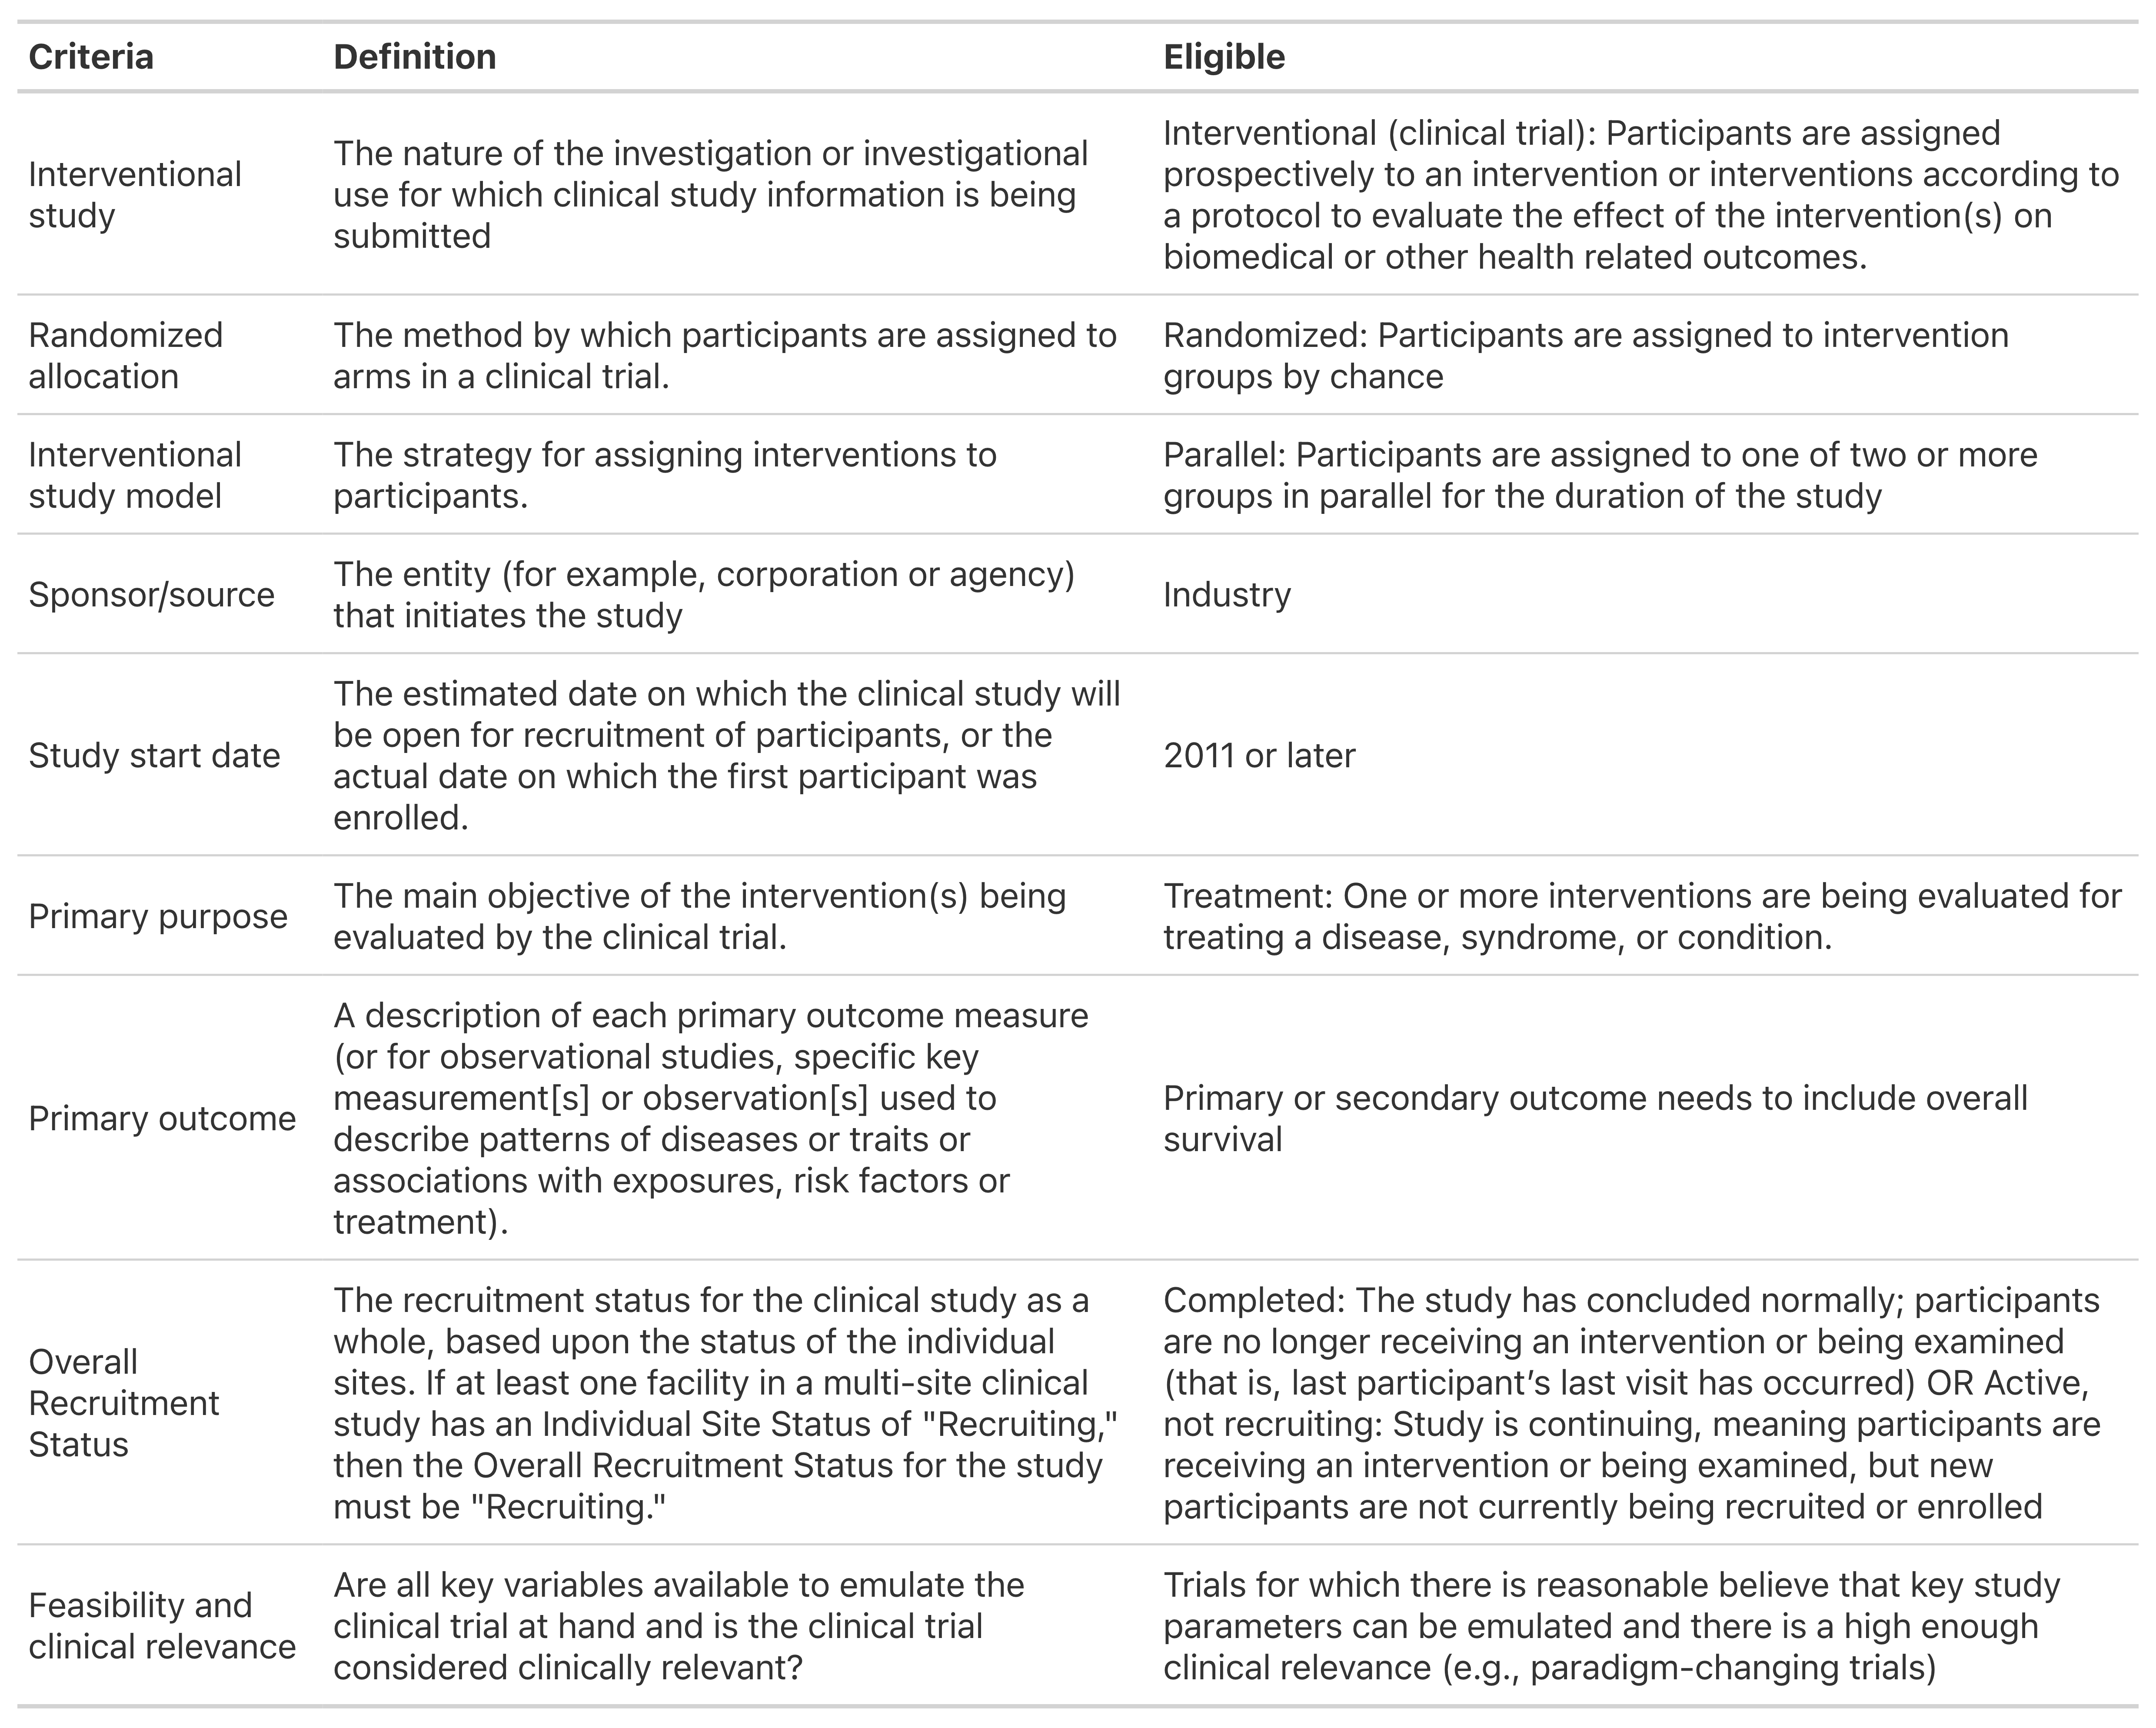
\includegraphics[keepaspectratio]{../tables/Table_1_trial_eligibility.png}}

}

\end{table}%

\newpage{}

\begin{table}[h]

\caption{\label{tbl-rcts}Tentative list of randomized controlled trials
(RCTs) considered for emulation.}

\centering{

\pandocbounded{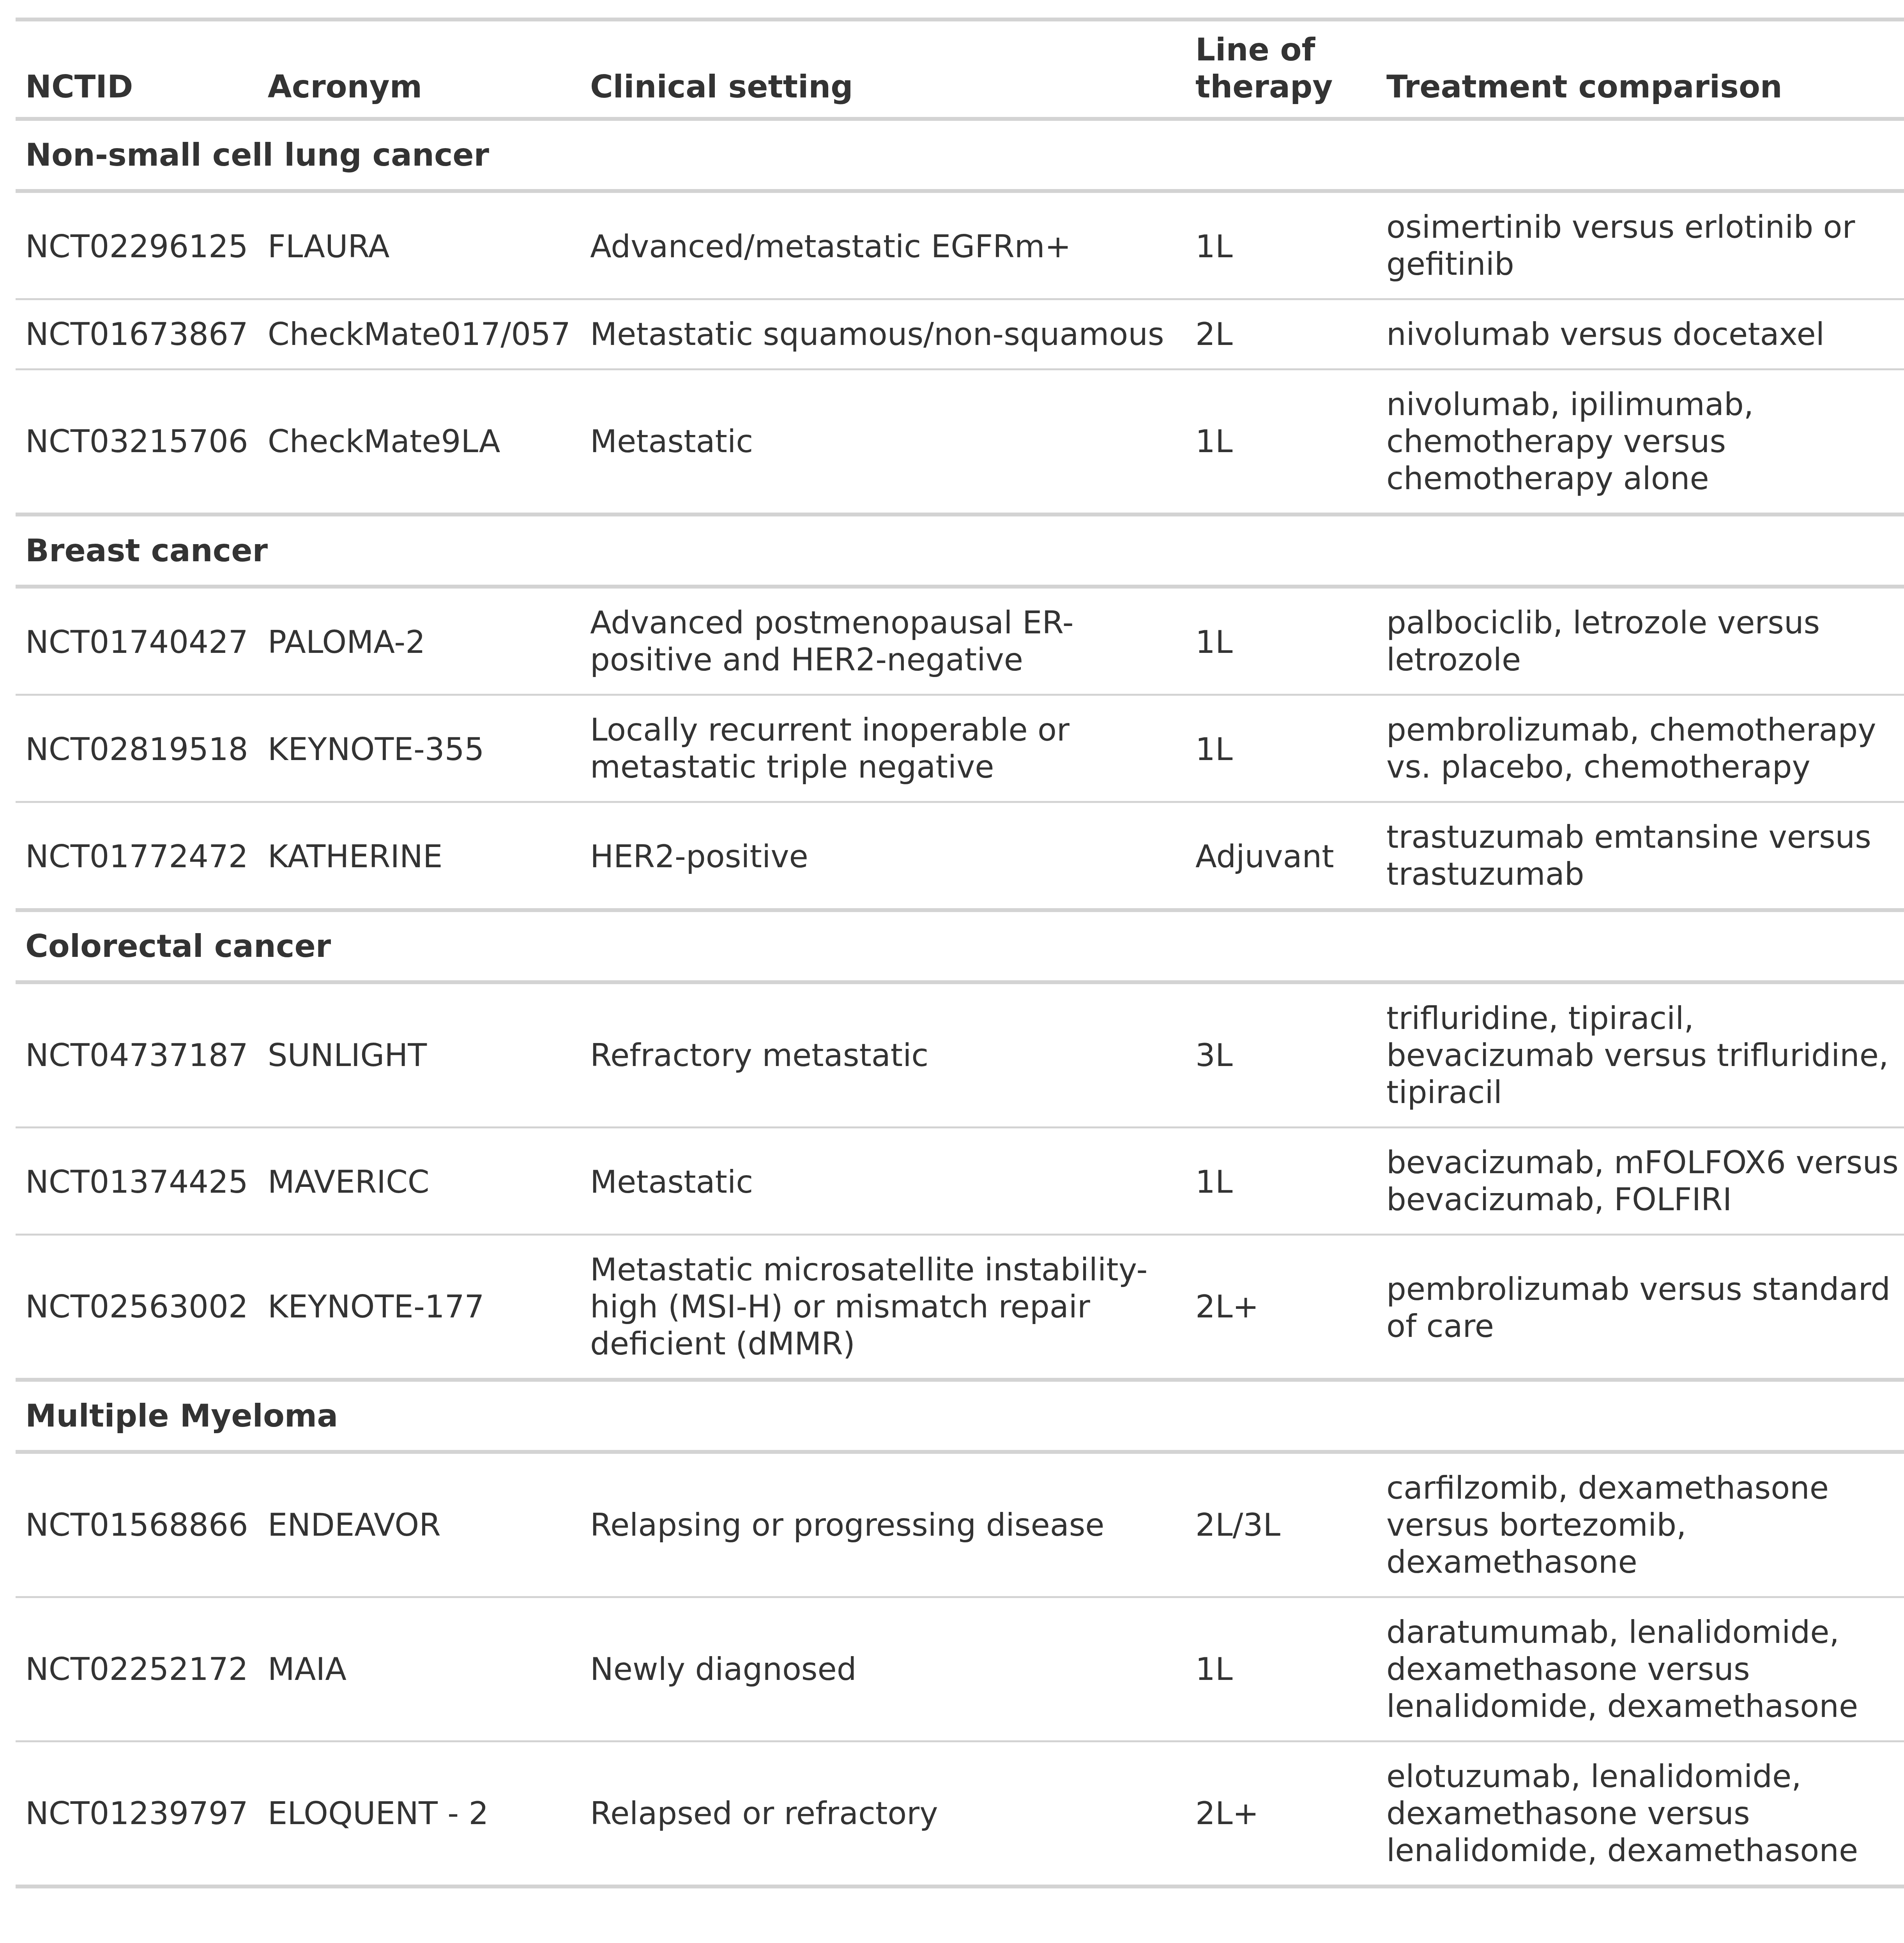
\includegraphics[keepaspectratio]{../tables/Table_2_trial_selection.png}}

}

\end{table}%

\newpage{}

\begin{table}[h]

\caption{\label{tbl-metrics}Example visualization of agreement metrics.}

\centering{

\pandocbounded{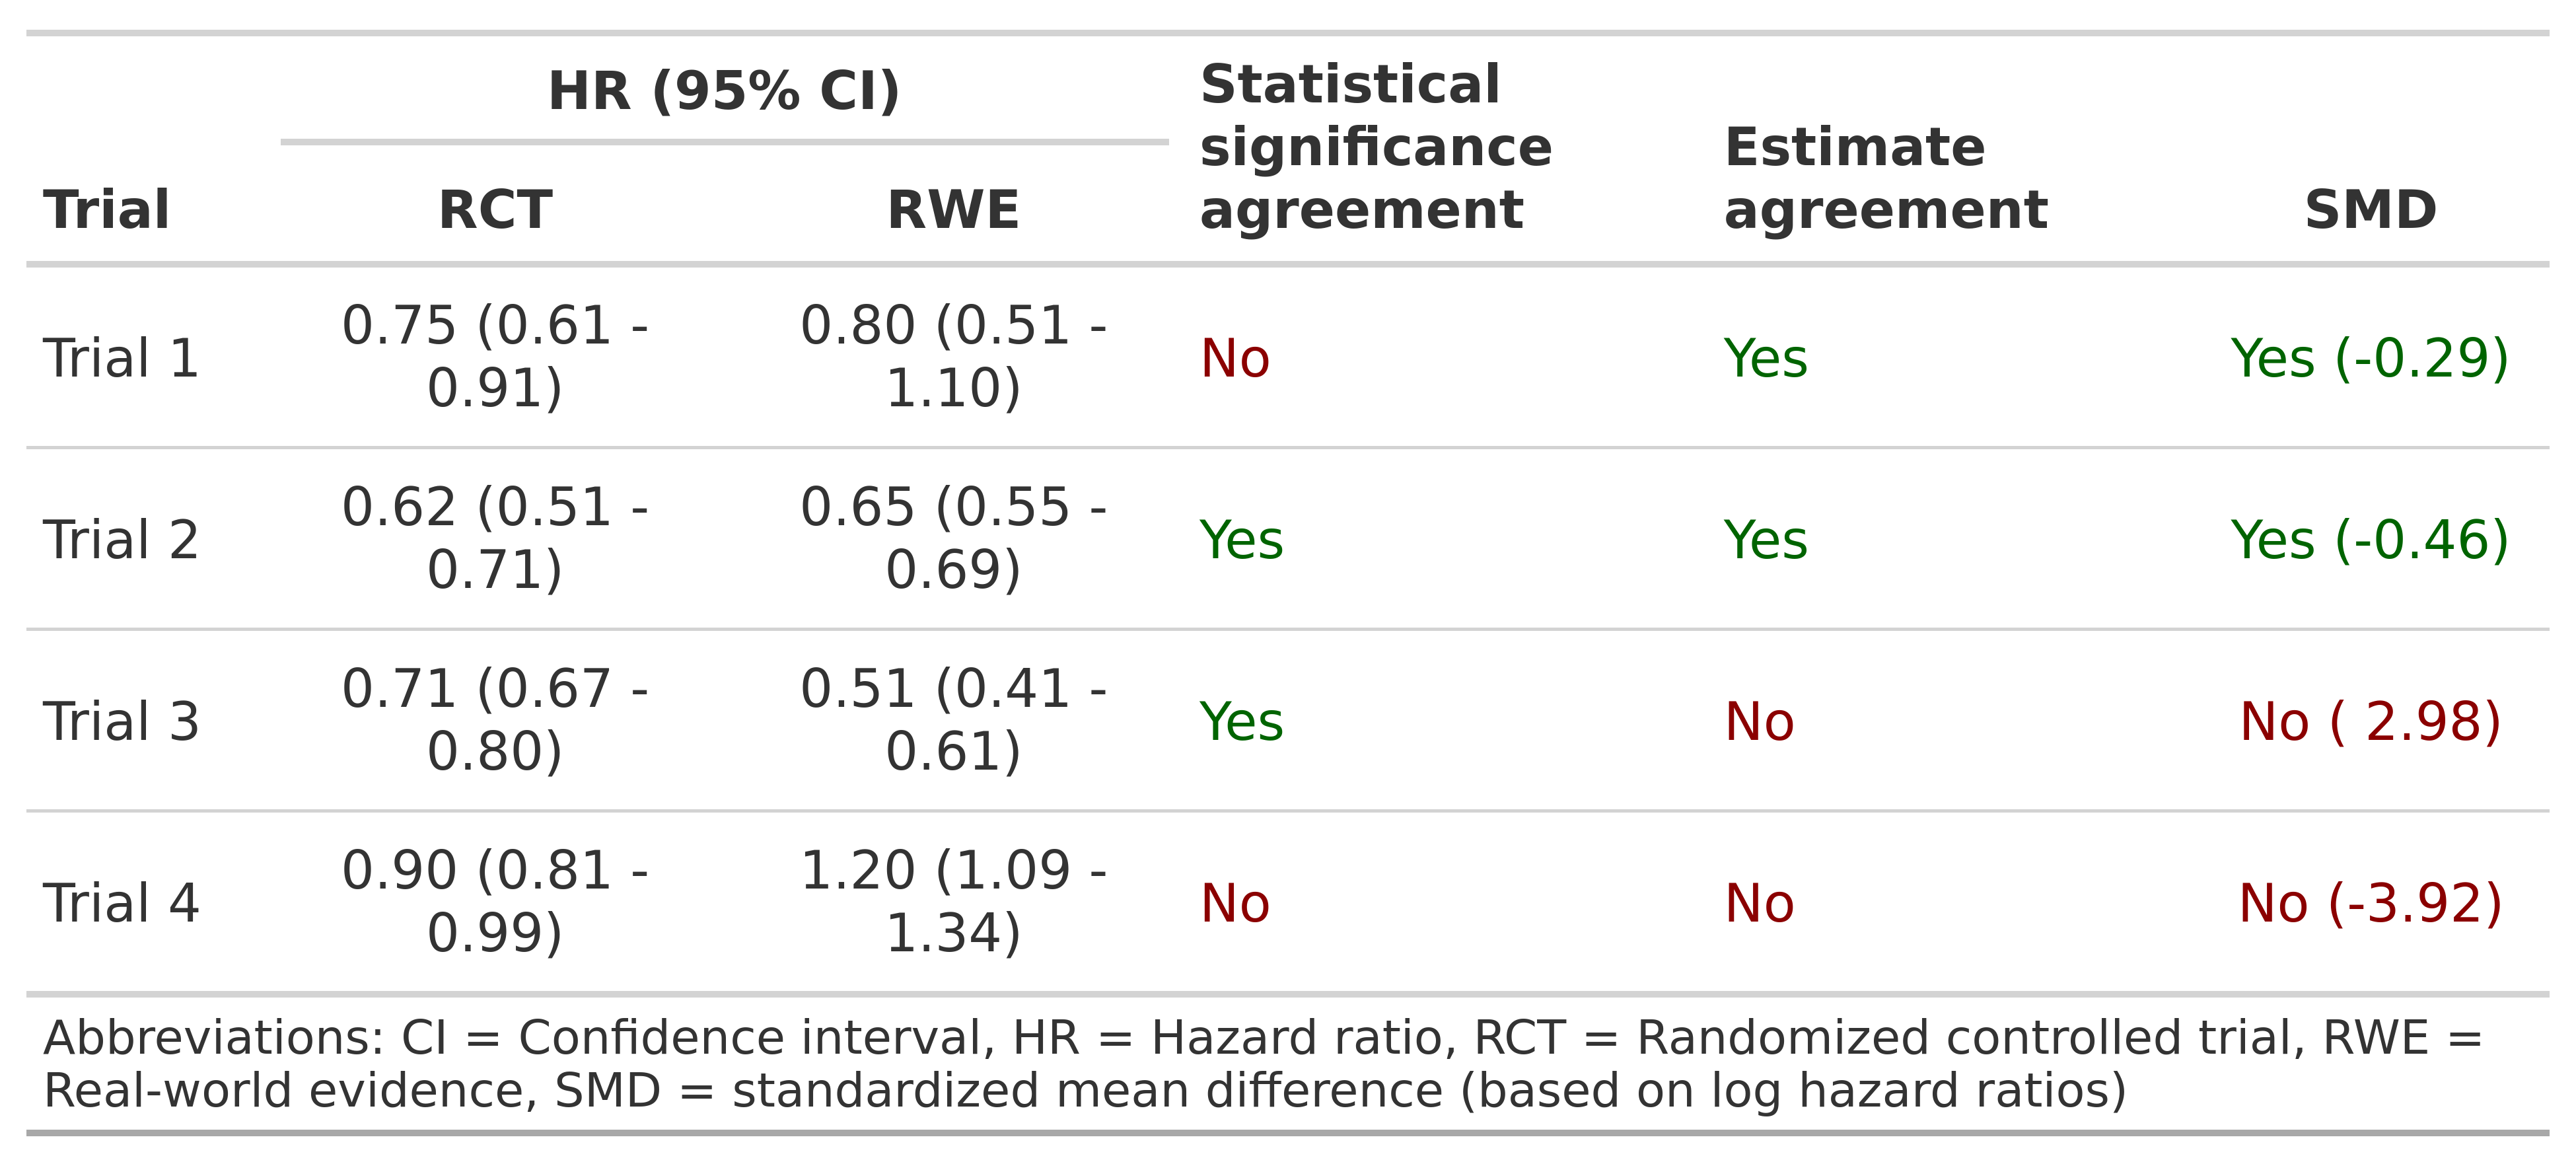
\includegraphics[keepaspectratio]{../tables/Table_3_agreement_metrics.png}}

}

\end{table}%

\newpage{}

\section*{Figures}\label{figures}
\addcontentsline{toc}{section}{Figures}

\begin{figure}[h]

\caption{\label{fig-process}Systematic process to understand
effectiveness claims of oncology trials using real-world evidence.}

\centering{

\pandocbounded{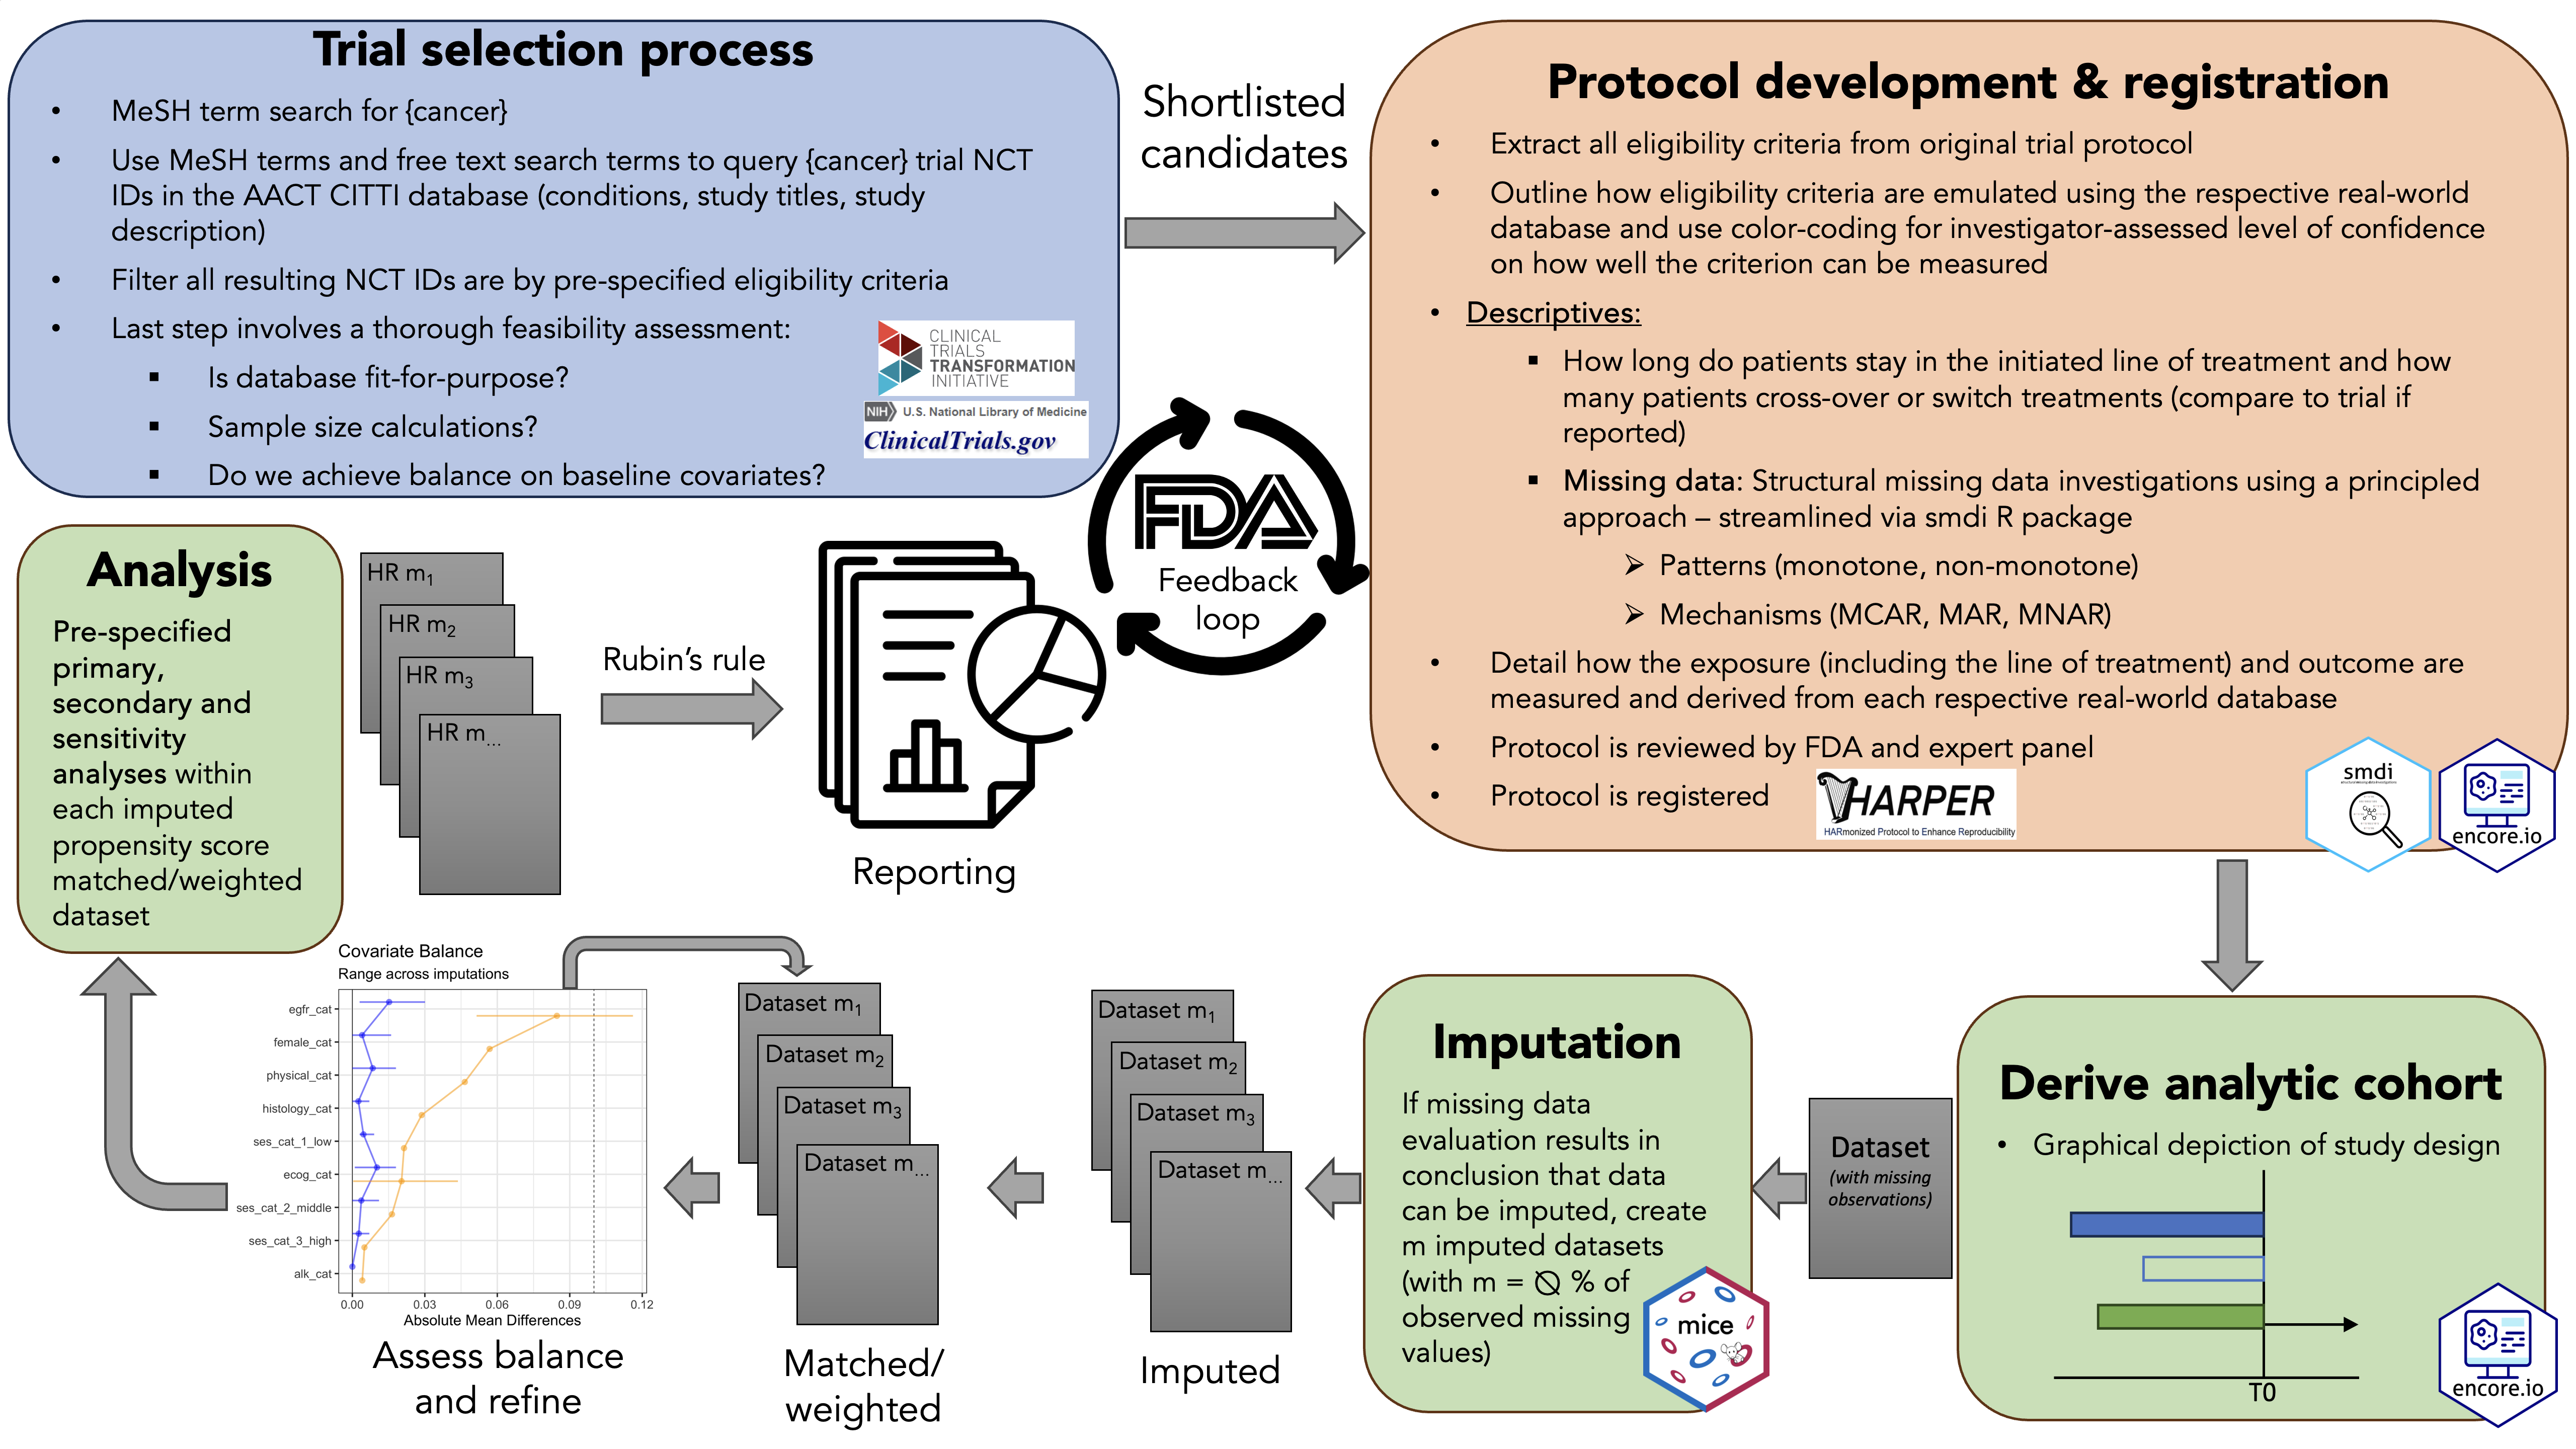
\includegraphics[keepaspectratio]{../figures/process.png}}

}

\end{figure}%

\newpage{}

\begin{figure}[h]

\caption{\label{fig-initiators}Example visualization of descriptive drug
utilization analyses displaying a) initiation trends between compared
regimens based on calendar time, b) cumulative rate of patients
switching to another line of treatment.}

\centering{

\pandocbounded{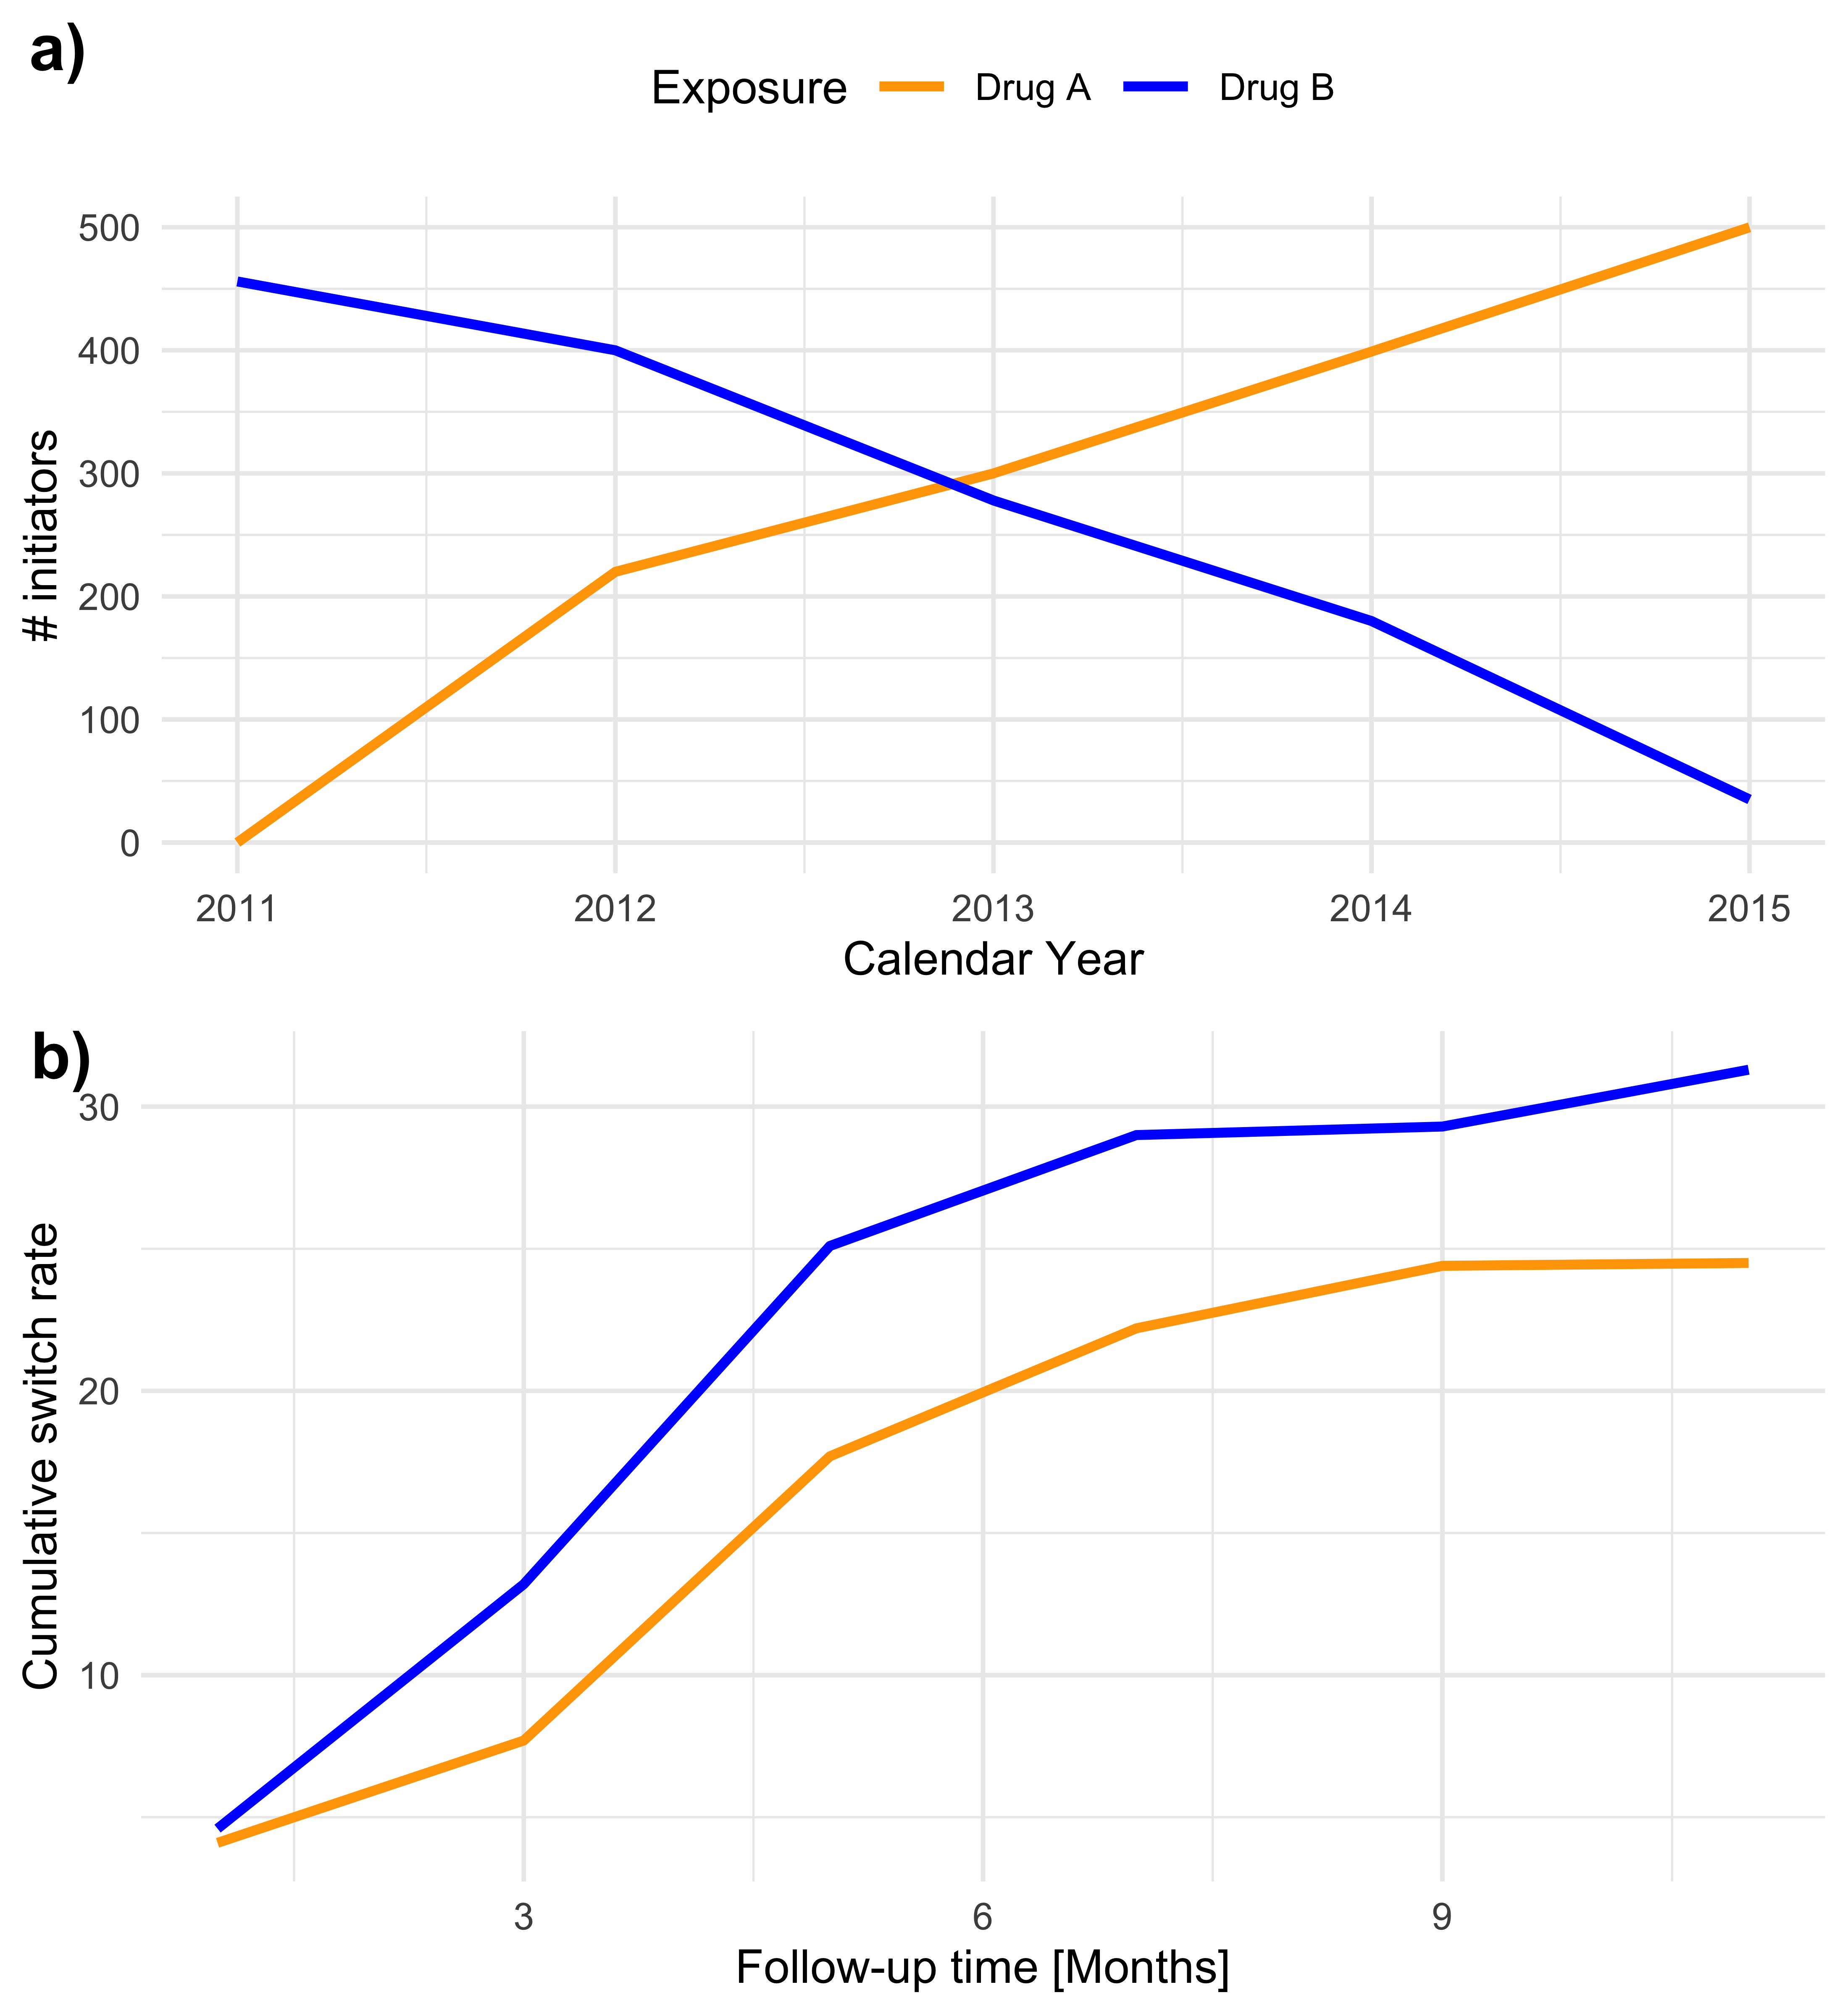
\includegraphics[keepaspectratio]{Figure_2_utlization.png}}

}

\end{figure}%

\newpage{}

\begin{figure}[h]

\caption{\label{fig-balance}Assessment of a) covariate balance and b)
distributional balance of a prognostic score for overall survival before
and after propensity score matching or weighting across multiple imputed
datasets.}

\centering{

\pandocbounded{\includegraphics[keepaspectratio]{Figure_3_balance.png}}

}

\end{figure}%




\end{document}
